\documentclass{article}
\usepackage[utf8]{inputenc}
\setlength{\parskip}{1em}
\usepackage{subcaption}
\usepackage{csvsimple}
\usepackage{graphicx}
\usepackage{lscape}
\usepackage{longtable}
% Please add the following required packages to your document preamble:
\usepackage{booktabs}
\usepackage{longtable}
\usepackage{tabularx}
\usepackage{pdflscape}
\usepackage{afterpage}
\usepackage{capt-of}% or use the larger `caption` package

\usepackage{biblatex}
\addbibresource{Chapter_2/reference.bib}

\title{Chapter 1}
\author{Jonathan S. Abrahams }
\date{October 2019}
%\usepackage{natbib}
\usepackage{graphicx}
% Please add the following required packages to your document preamble:
\usepackage{lscape}
\begin{document}

\maketitle

\section{Introduction}
%Three major comments on this chapter:
%1. Need a tree for ASR
%2. More details about the strains used for the B1917 tree
In addition to deletion and rearrangement, IS-mediated recombination can result in duplication. Twelve copy number variants (CNVs) in B. pertussis have been described and studies with sufficient genomic data have resolved them as tandem repeats. Duplication of a region containing cyaA (encoding adenylate cyclase-haemolysin) increased haemolytic activity and it was noted that this duplication was highly unstable. These serendipitous observations suggest that CNVs are a poorly characterised contributor to genetic diversity among B. pertussis. However, to date there has been no systematic analysis of CNVs in B. pertussis and indeed systematic analysis of structural variants at the species level is rare for bacteria, although it is relatively common in Eukaryotic organisms. In this chapter I sought to create a generic method to catalogue CNVs in B. pertussis, utilising publicly available genomic data, which is overwhelmingly derived from short-read sequencing platforms. 

\section{Results}

\subsection{Duplications in a set of genomes}

The US Centers for Disease Control and Prevention (CDC) conducts routine and enhanced surveillance of pertussis, which includes whole genome sequencing of B. pertussis clinical isolates using combinations of data from: PacBio, Illumina,Nabsys and Opgen platforms.  A hybrid assembly process is used on these isolates and is able to produce closed genomes for the vast majority of strains\cite{WhoopingGenomeEpidemicsc}. There is, however, a minority of strains that fail this process (assemblies producing >1 contig). MW scrutinised these further for genomic anomalies and confirmed them with Nabsys sequencing\cite{Weigand2018ScreeningPertussis/ie}

Some of these strains revealed increased read depth coverage localized to discrete genomic regions (Figure \ref{fig:CDC_isolates_coverage}). Manual resolution of the putative CNV was attempted if such spikes were detected.

\begin{figure}[h!]
\centering
\includegraphics[width=\textwidth{}]{"Chapter_1/big coverage CDC".png}
\caption{An example of a large spike in read coverage. Such spikes were accompanied by a failure of PacBio assemblies to close the genome and further investigation into these genomes resulted in each having a CNV at the spike in coverage.}
\label{fig:CDC_isolates_coverage}
\end{figure}

When reads longer than the longest repeat in the genome are assembled, a closed genome can be easily made. In cases where CNVs were detected in BP,however, the repeats were much longer than the longest PacBio reads, which are at maximum 30kb. Enzyme mapping was therefore performed which produces DNA fragments of 0.15Mb-1Mb in size.

At the time of writing there is no simplified method to combine Illumina, PacBio or Nabsys reads and optical maps. This data was therefore used to inform MW of the likely genome structure. This was done by using the enzyme maps to create a hypothetical genome structure in-sillico and subsequently mapping the PacBio reads to the new structure in order to prove the hypothesis to be true. If the resulting mapped reads reveal no gaps or errors, the right genome structure was found.

Using this methodology, genomes from 28 strains, including two used for the production of vaccines against pertussis, were resolved with one CNV each. Some of these CNVs were large (>300kb), involving hundreds of genes (Figure\ref{fig:CDC_isolates}).

This dataset has a number of immediately recognisable characteristics, which are repeated in the large independent data set throughout this chapter: A non-random and clustered distribution on the genome; variable gene content within a cluster and variable length of CNVs but often over 50kb. These trends are highlighted in Figure \ref{fig:CDC_isolates}).

\begin{figure}[hbtp]
\centering
\includegraphics[width=\textwidth{}]{"Chapter_1/combined figures12341".jpg}
\caption{The genomic loci, in relation to B1917, that had undergone copy number change (without being effected by rearrangement) were plotted for the 25 genomes (A). CNVs longer than 50kb are coloured red. A closer look at the CNVs indicated by the blue box in (A) is provided in (B)- it can be clearly seen that the CNVs have varying gene contents.}
\label{fig:CDC_isolates}
\end{figure}

Using the manually resolved dataset as a benchmark, we sought to develop a prediction and screening tool to identify CNVs within the public repository of B. pertussis genome sequence data on the Sequence Read Archive (SRA) using a scalable and automated approach.

\subsection{Read depth- pros and cons of different read depth tools}
Because the copy number of a locus is beyond the resolution of short read data, it is necessary to use other sources of data as proxies. There are a number of these types of proxies that can be used, but the most fundamental and informative is the read depth. The logic is simple: more copies of a locus will mean higher numbers of reads that map to this region in the reference genome (Figure \ref{fig:Schematic_graph}).

Split read signals (a read spanning a SV junction) and read-pair data (measuring the distance between read pairs) are an additional data source that can be used to predict CNVs. Such data can provide base pair resolution to the breakpoints. Both methods,however, rely on the CNV breakpoint to not be in a repeat region that is larger than the read size. This is therefore not applicable to B.pertussis, and this data is demonstrably absent in the CNVs described here (Figure \ref{fig:Close_but_no_cigar}), where CNVs are flanked by repeat regions exceeding 1kb in length- beyond the resolution of short reads which are upto 300bp in length. 


\begin{figure}[h!]
\centering
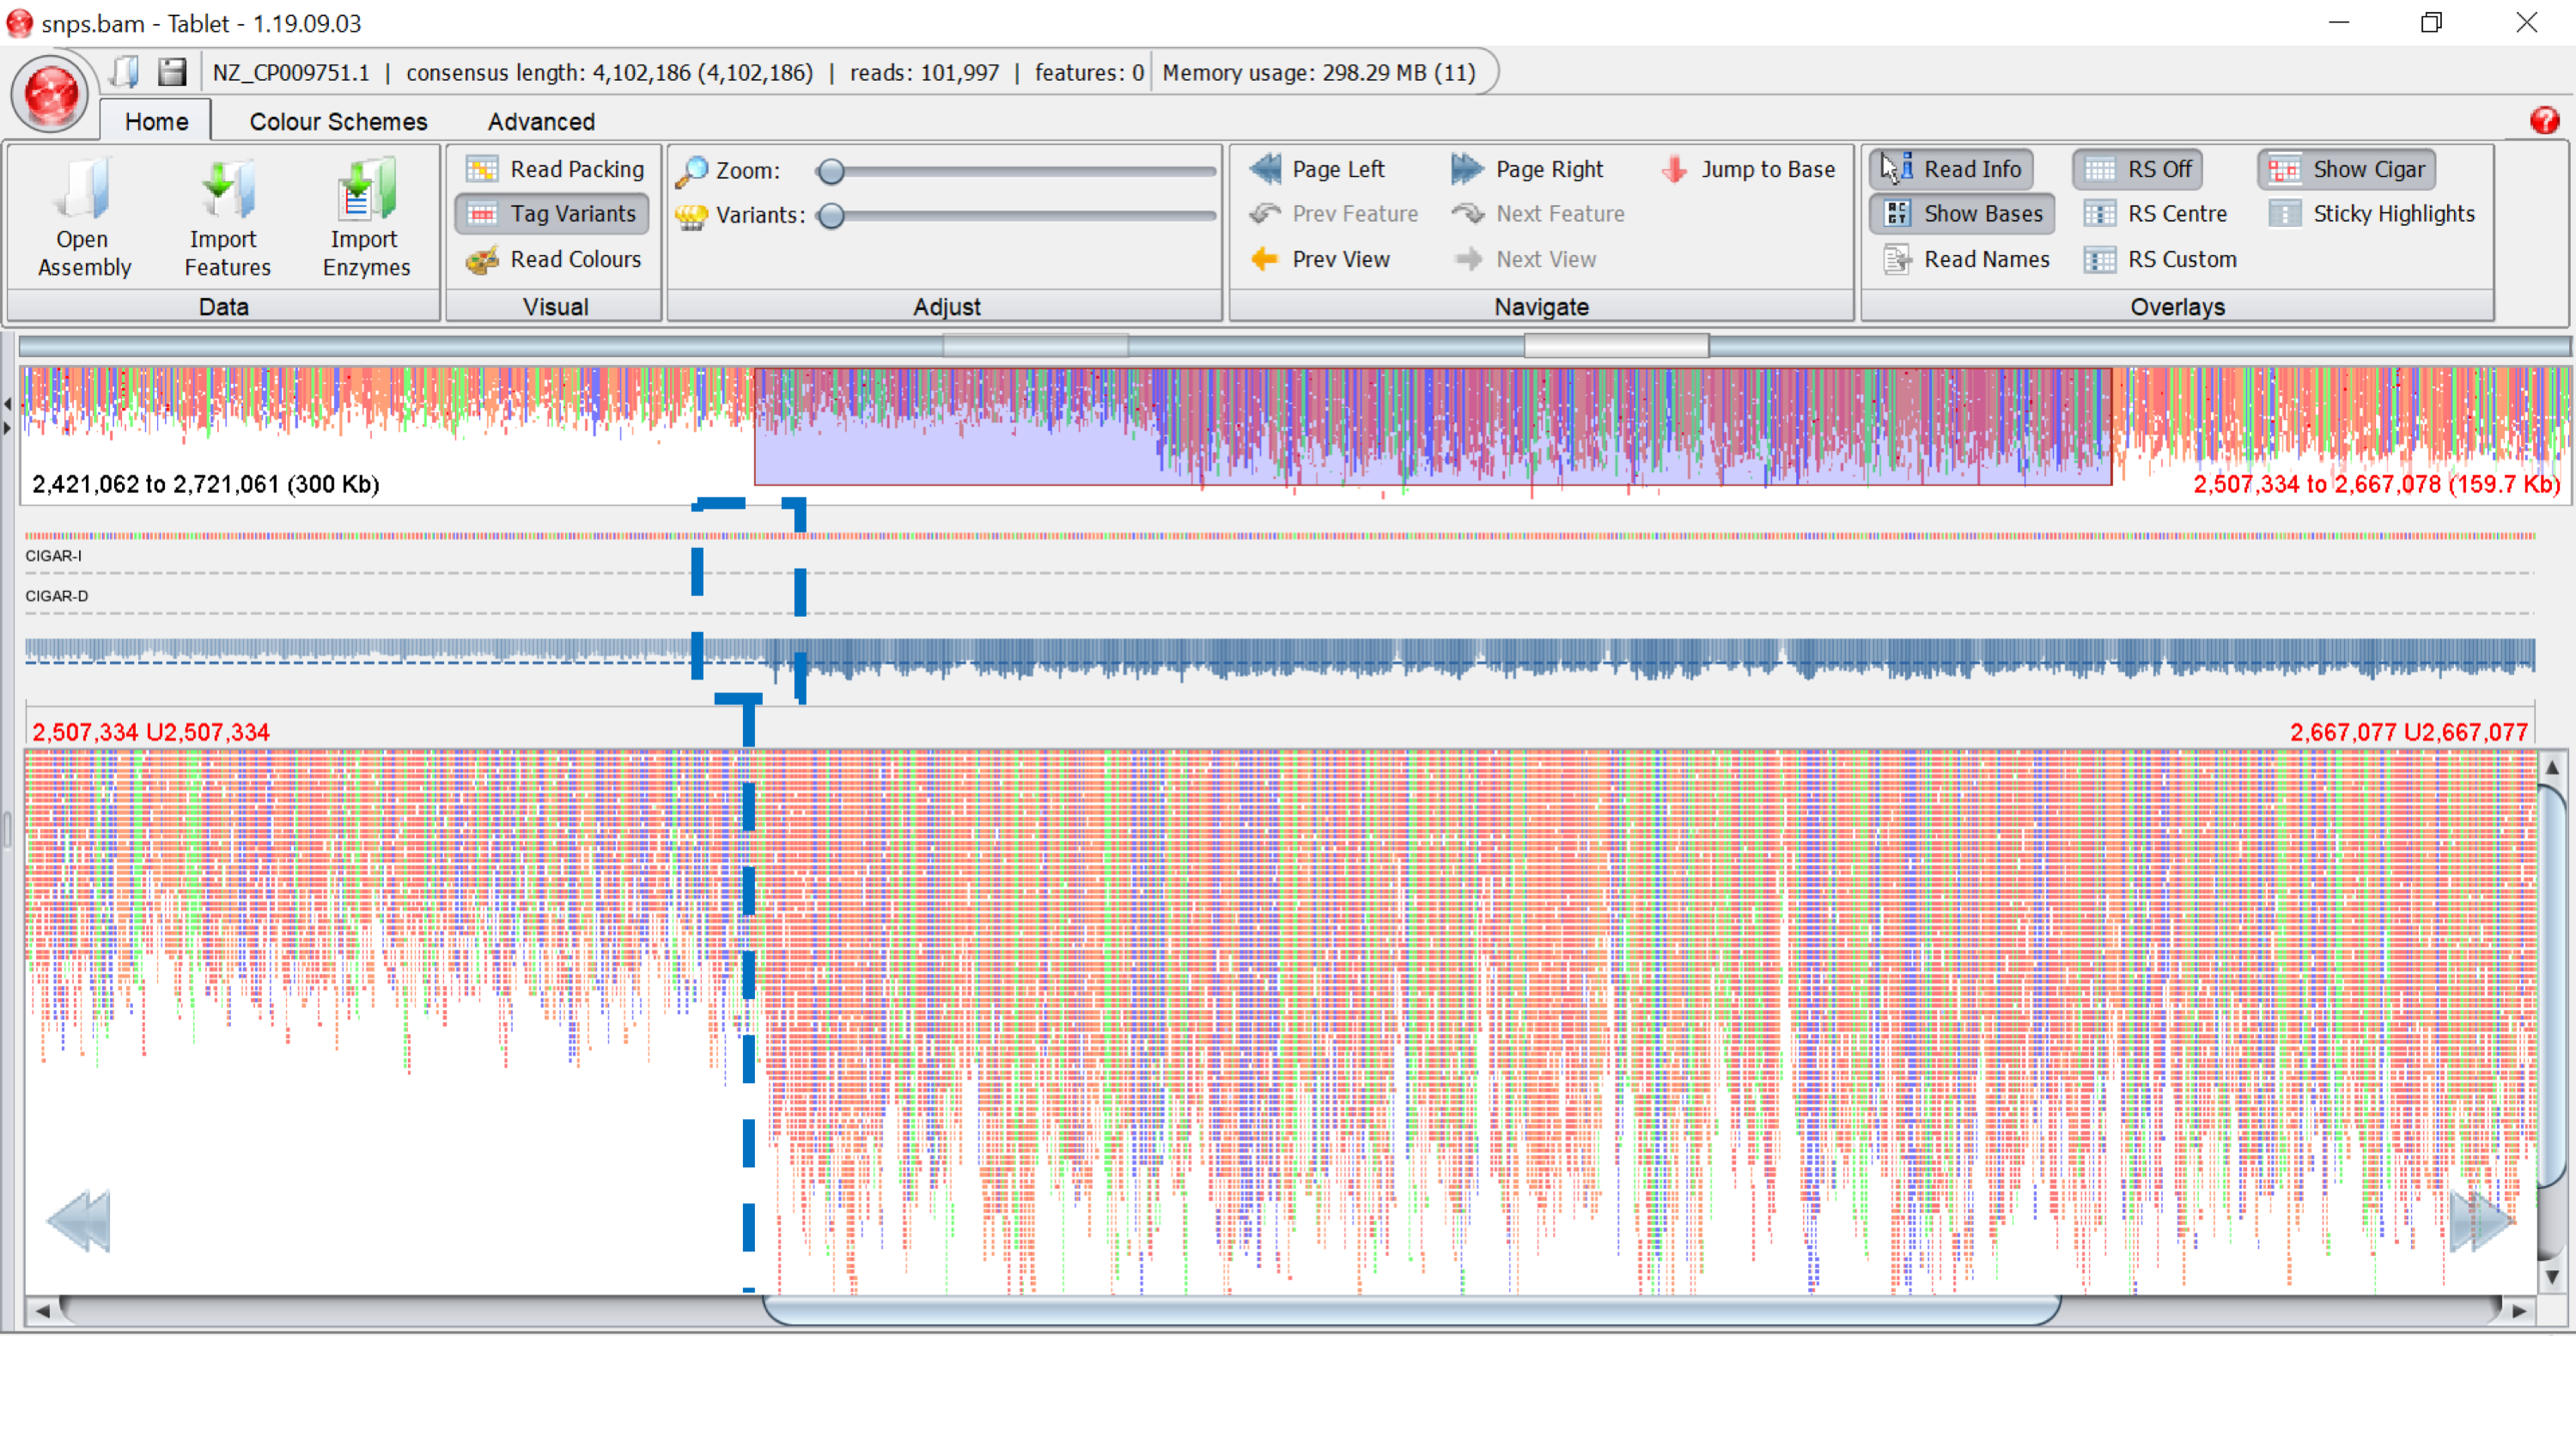
\includegraphics[width=\textwidth{}]{Chapter_1/tablet.png}
\caption{The genome of UK48 was mapped to B1917 and the alignment viewed in tablet. A clear increase in read depth can be seen(to the right of the blue dashed line), yet, no signal was seen in the cigar string (no reads flagged in the blue box)}
\label{fig:Close_but_no_cigar}
\end{figure}


\begin{figure}[h!]
\centering
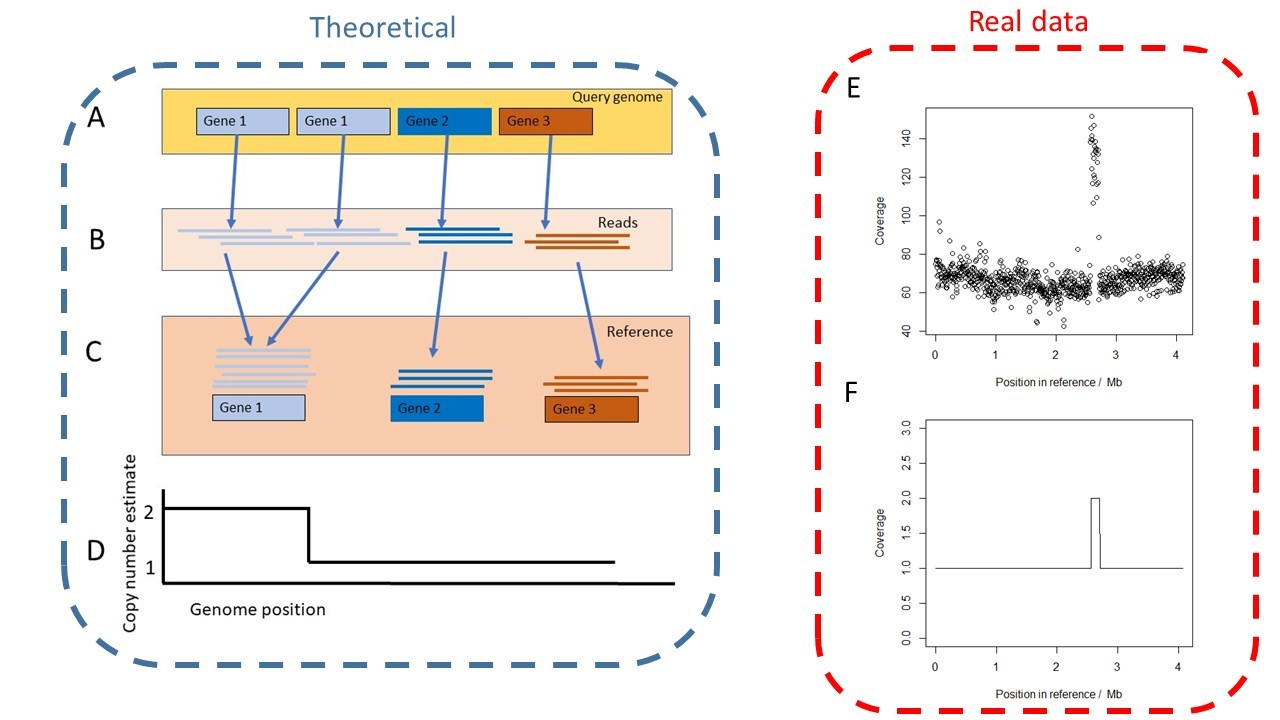
\includegraphics[width=\textwidth{}]{Chapter_1/intro ting.jpg}
\caption{. Schematic overview of prediction of CNVs from sequencing read depth. In the theoretical example (purple box, left), the query strain contains a perfect tandem duplication of gene 1 whilst gene 2 and 3 are at single copy (A). Short reads from the query strain are generated (B) and mapped to the reference genome, that contains all genes at single copy (C). Reads from both copies of gene 1 in the query strain map to this locus in the reference sequence and thus twice as many reads map to this gene compared to genes 2 and 3. This data must be processed to avoid technical bias, the pipeline processes read coverage data into estimates of copy number (D). Using an example with real data (red box, right) the strain SAMN08200079 was analysed. Read coverage was graphed to reveal a duplication at ~1.4Mb (E, analogous to theoretical graph C) -an example of a statistical analysis of this data was then graphed (F, analogous to theoretical graph D).  }
\label{fig:Schematic_graph}
\end{figure}


\subsubsection{How window length effects CNV predictions}

Predicting CNVs in data sets of bacterial genomes which are frequently hundreds to thousands of small genomes, rather than fewer but larger genomes for eukaryotes, presents a challenge- one that is not often mentioned in the literature. Comparing coverage data across 1000's of samples which vary by a multitude of factors such as sequencing chemistry, sequencing instruments and read lengths is complex and causes fluctuations in coverage. It is not known, however, exactly which combination of factors contribute to the inter-sample differences in read coverage.


%Probably need to normalise the Y axis
\begin{figure}[h]

\includegraphics[width=\textwidth{}]{Chapter_1/"read depth figures".png}
\caption{Reads were mapped to the reference genome for three isolates and the average read depth plotted in 5kb windows. Genomes A, B and C show low,medium and high read depth noise respectively.}
\label{fig:Schematic_graph}
\end{figure}

Because read depth is the proxy used here for predicting CNVs, artefactual fluctuations in read depth can appear as false positive CNVs in the analysis. It is therefore necessary to normalise these fluctuations. All read depth based prediction tools will analyse the read depth in windows to analyse how read depth changes across the genome. However, the size of this window influences the results. Larger windows are less sensitive to fluctuations in read depth but are also very specific (low false positives) whilst the inverse is true for smaller windows. Therefore larger windows can be used on genomes with high read depth fluctuations and smaller windows for less noisy genomes. CNVnator provides extensive supplementary data and methods pertaining to this and notes a heuristic: The optimum ratio of average read depth to the standard deviation is generally between 4-5 \cite{Abyzov2011CNVnator:Sequencing}. Choosing window size, therefore, is a balancing act of these factors.

%The 25 manually resolved genomes were all too good quality to assess the effectiveness of varying the window length.
%Therefore simulated data was appropriate.
%How window length effects SD was simulated
%I generated fake coverage data of 100x coverage with sd of 5,10,20 and 50.  THis was based on noisy data I found using BP.

\subsubsection{Why B1917 for mapping}

The choice of reference is important when using a mapping pipeline. Although the pangenome of BP is small \cite{Park2012ComparativePathogensc}, any gene that is not present in the reference will not be analysed in the mapped data. Additionally, and much more relevant for BP, when data is mapped to a reference the true gene order of the sample is masked. Therefore, strains with duplications in rearranged loci may appear as discontinuous stretches of duplicated DNA in the reference-obscuring the true genomic structure of the CNV.

To minimise the side-effects of read mapping, therefore, an isolate that was broadly representative in terms of gene content and gene order was needed. Additionally, the strain must be widely used so that any results can be tested and replicated by the scientific community. It is known that the strain B1917 is generally representative of the gene content of recent circulating isolates and has been recently established as a modern reference genome, thus leading to many labs having a stock of it. It is therefore the only viable alternative reference genome to Tohama. 


%Check these numbers are correct. Potentially expand the numbers, upto ~20

It was not clear,however, if B1917 had a representative gene order and therefore a brief demonstration to prove this was undertaken. A whole genome alignment was conducted with 3 of the test genomes, B1917\cite{Bart2014CompleteLineages}, Tohama\cite{Parkhill2003ComparativeBronchiseptica.} (the customary reference genome that was isolated in the 1950's) and 2 closed genomes,isolated outside of the USA in recent outbreaks \cite{Dienstbier2018ComparativePertussis},\cite{}, for a broader comparison.



\begin{figure}[h!]
\centering
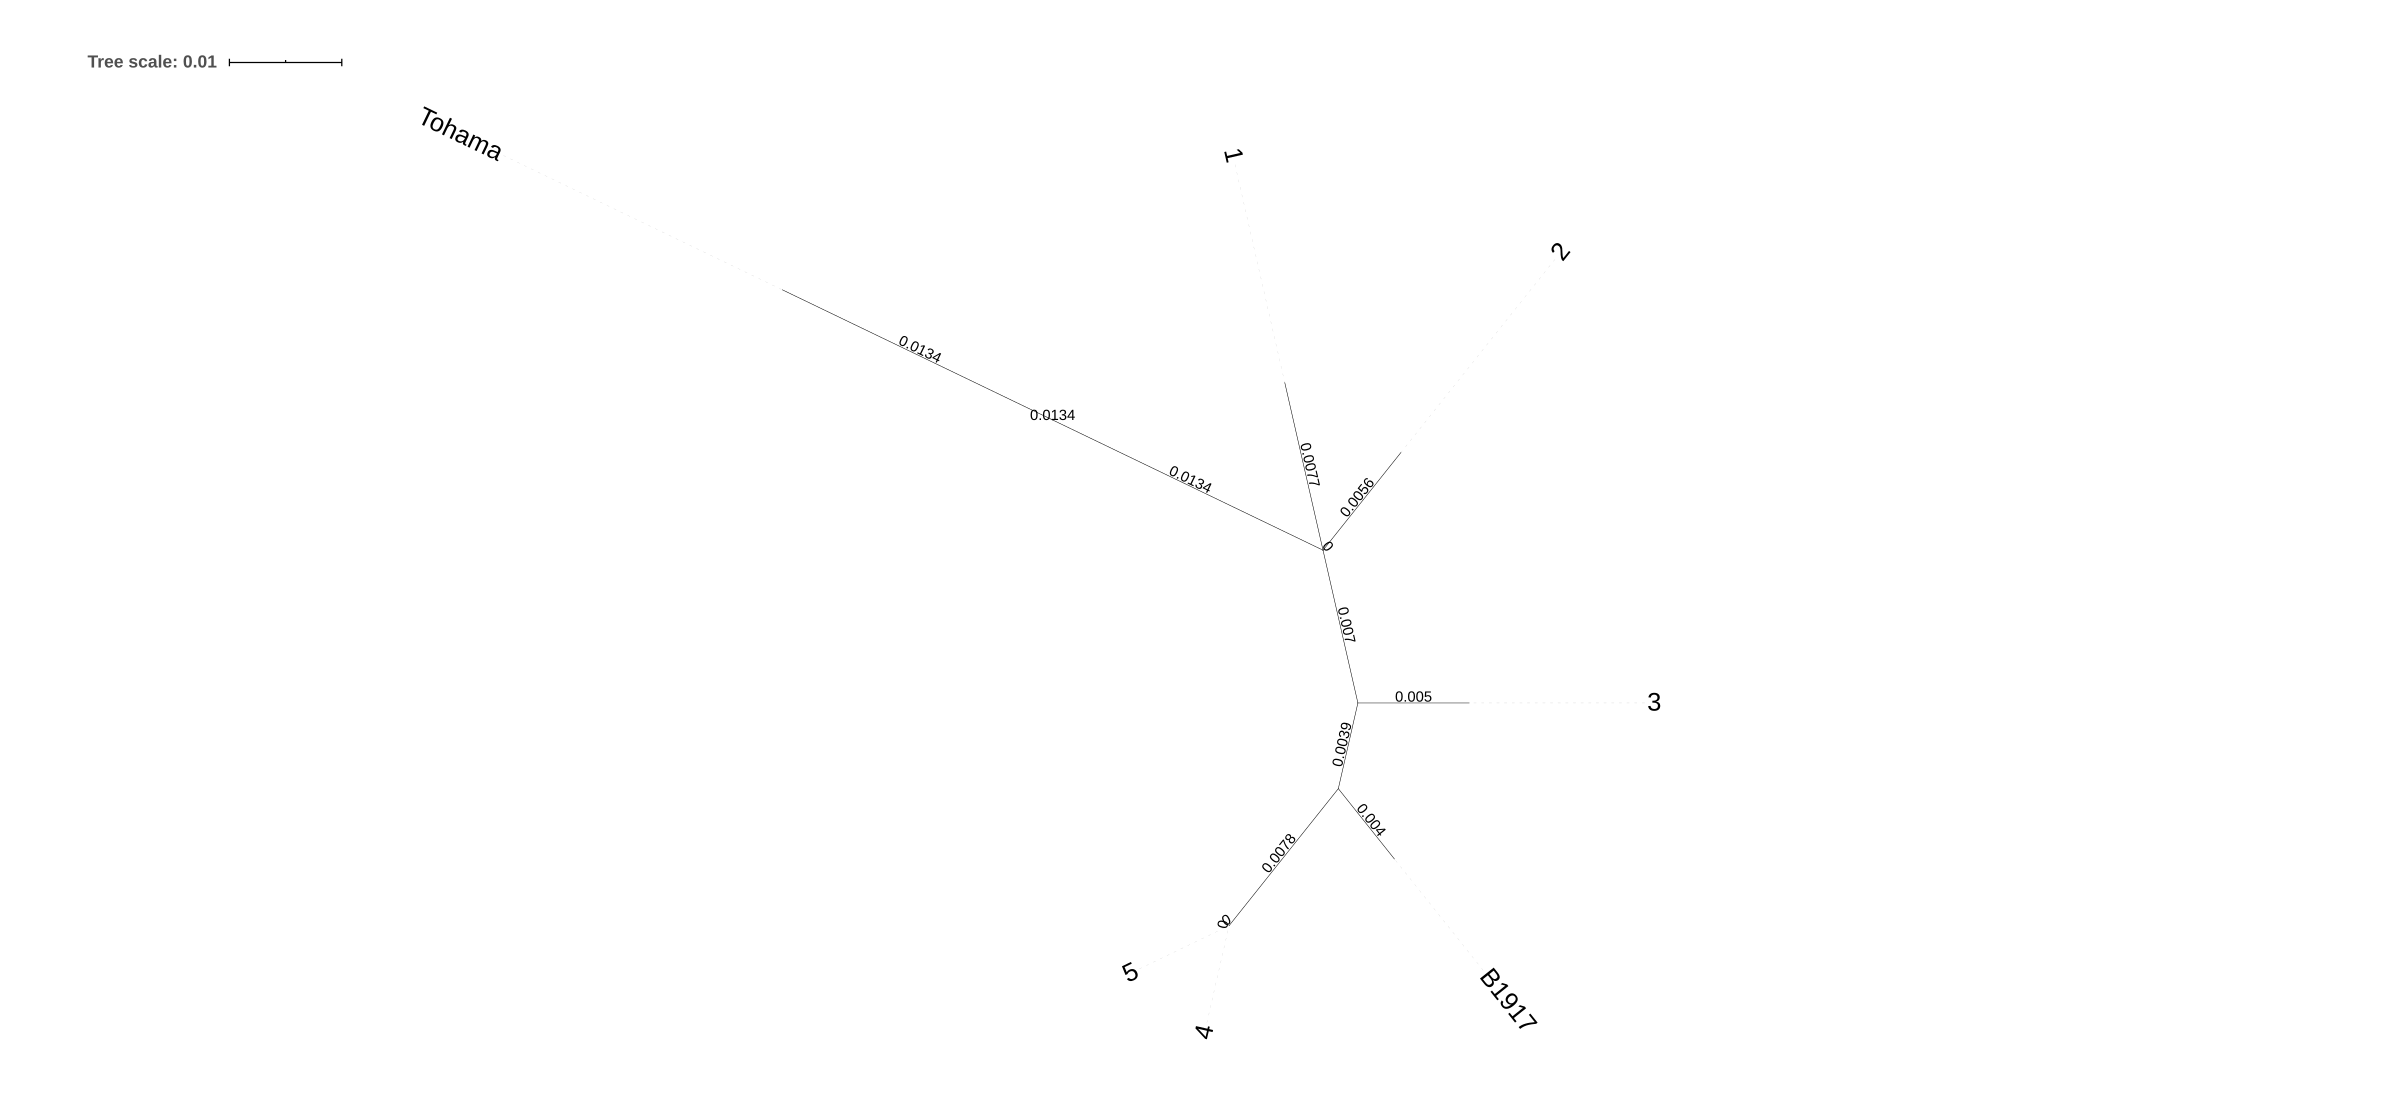
\includegraphics[width=\textwidth{}]{Chapter_1/VwSDoN3HlH4ng9uLHTKImg.png}
\caption{A test tree showing that Tohama is separated by roughly 3x as many unique gene order changes (branch length: 0.013) from the rest of the phylogenetic tree as compared to B1917 (branch length: 0.004). This demonstrates that B1917 has a gene order that is closer to modern isolates}
\label{fig:Gene_order_tree}
\end{figure}

The tree of gene order changes shows that B1917 was separated by less gene order changes to all isolates in the dataset compared to Tohama. B1917 is therefore the most appropriate reference genome. 

\subsubsection{Training dataset -B1917}

The first verification that CNVnator could produce reliable results was to simulate short read data for the B1917 reference genome and to establish that no false positives were detected.

The performance of our approach was tested using Illumina HiSeq reads simulated from the B1917 reference genome. As expected, no CNVs (false positives) were predicted and all genes were correctly estimated at single copy. 

The approach was subsequently evaluated by analysing the set of 28 manually resolved genomes.

\subsubsection{Manually resolved genomes }

When establishing the accuracy of the pipeline I first considered resolved CNVs that were contiguous on the B1917 reference genome. This is because read-depth is theoretically limited to simple CNVs compared to these complex CNVs which contain multiple SVs at the same locus. Two samples were therefore analysed separately as they contained complex CNVs. Whilst the 25 simple CNVs mainly occurred at  three distinct loci, their beginning and ending coordinates, as well as overall length, varied between strains. Thus, three measures of accuracy were tested: the correct prediction of the 25 CNVs, the quantity of false positives and the discrepancy in the start/end loci between the predicted and true CNVs (breakpoint accuracy). Only one (J321) of the 25 data sets failed our quality control (see Methods) for high read depth noise and was excluded; leaving 24 high quality strains.



\begin{figure}[h!]
\centering
\includegraphics[width=\textwidth{}]{Chapter_1/"copy number comparison".jpg}
\caption{The discrepancy between the copy number estimates from CNVnator (orange) and the resolved copy numbers (blue) are highlighted.}
\label{fig:CDC_copy_number_discrep}
\end{figure}

%CNVnator
Of the 24 resolved, high quality and suitable CNVs, 23 were correctly predicted (defined as >=80\% reciprocal overlap) (Table \ref{tab:CDC_vs_me}). Three false positives were detected in three different strains. Two of these were due to one gene within the CNV locus being predicted as single copy, causing the true, single CNV to be predicted as two, separated by the falsely predicted single copy gene.  In the third false positive, a second locus was predicted as a duplication and whilst mapping PacBio reads to the reference also showed increased coverage at the same locus, enzyme mapping showed no evidence of a second duplicated locus in this isolate. 

The breakpoint accuracy of estimates was calculated with false positives excluded (Figure \ref{fig:CDC_breakpoint}). The median distance between the true values and the read depth-based estimates was 0.5 genes. There were five estimated start/end points which were considerably (>=5 genes) less accurate than the rest of the dataset, mainly arising from the two strains in which the CNV was predicted as two separate loci.

Thus the pipeline correctly predicted, and with excellent breakpoint accuracy, the CNVs for 20 of the 27 resolved genomes (74\%), with 3 further correctly CNVs predicted (11\%) but as two adjacent but separate loci.

\begin{figure}[h!]
\centering
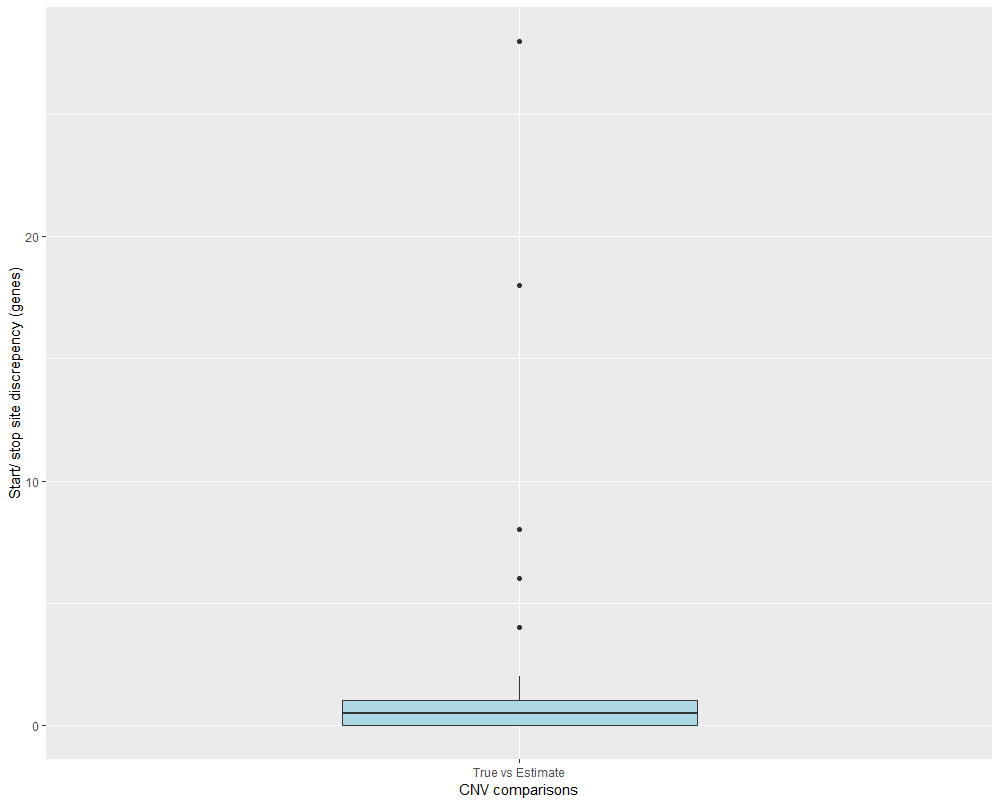
\includegraphics[width=\textwidth{}]{Chapter_1/cdc_supp_b.png}
\caption{The discrepancy of both the start and end breakpoints of the 23 true positive predictions to their respective resolved duplication was analysed as a boxplot. This showed a tight distribution around the median distance  of 0.5 genes discrepency.}
\label{fig:CDC_breakpoint}
\end{figure}


% Please add the following required packages to your document preamble:
% \usepackage{graphicx}
\afterpage{%
    \clearpage% Flush earlier floats (otherwise order might not be correct)
    \thispagestyle{empty}% empty page style (?)
    \begin{landscape}% Landscape page
        \centering % Center table
\begin{table}[]

\resizebox{\textwidth}{!}{%
\begin{tabular}{lllllllllllllll}
\hline
CNV Index & Alias & Accession & Estimate start (B1917 gene index) & Estimate end (B1917 gene index) & Estimated Length & Copy number estimate & True start (B1917 gene index) & True -Estimated start & True end (B1917 gene index) & True - Estimated end & True copy number & Copy\_number\_discrepency & Recip & False positive \\ \hline
\multicolumn{1}{|l|}{1} & \multicolumn{1}{l|}{J448} & \multicolumn{1}{l|}{SRR5071090} & \multicolumn{1}{l|}{2331} & \multicolumn{1}{l|}{2440} & \multicolumn{1}{l|}{109} & \multicolumn{1}{l|}{2.9} & \multicolumn{1}{l|}{2331} & \multicolumn{1}{l|}{0} & \multicolumn{1}{l|}{2440} & \multicolumn{1}{l|}{0} & \multicolumn{1}{l|}{2} & \multicolumn{1}{l|}{+/-0.2} & \multicolumn{1}{l|}{\textgreater{}=0.8} & \multicolumn{1}{l|}{N} \\ \hline
\multicolumn{1}{|l|}{2} & \multicolumn{1}{l|}{D236} & \multicolumn{1}{l|}{SRR9006092} & \multicolumn{1}{l|}{2798} & \multicolumn{1}{l|}{2947} & \multicolumn{1}{l|}{149} & \multicolumn{1}{l|}{1.7} & \multicolumn{1}{l|}{2799} & \multicolumn{1}{l|}{1} & \multicolumn{1}{l|}{2947} & \multicolumn{1}{l|}{0} & \multicolumn{1}{l|}{2} & \multicolumn{1}{l|}{Lower} & \multicolumn{1}{l|}{\textgreater{}=0.8} & \multicolumn{1}{l|}{N} \\ \hline
\multicolumn{1}{|l|}{3} & \multicolumn{1}{l|}{J737} & \multicolumn{1}{l|}{SRR9131607} & \multicolumn{1}{l|}{2798} & \multicolumn{1}{l|}{2947} & \multicolumn{1}{l|}{149} & \multicolumn{1}{l|}{2} & \multicolumn{1}{l|}{2799} & \multicolumn{1}{l|}{1} & \multicolumn{1}{l|}{2947} & \multicolumn{1}{l|}{0} & \multicolumn{1}{l|}{2} & \multicolumn{1}{l|}{+/-0.2} & \multicolumn{1}{l|}{\textgreater{}=0.8} & \multicolumn{1}{l|}{N} \\ \hline
\multicolumn{1}{|l|}{4} & \multicolumn{1}{l|}{J196} & \multicolumn{1}{l|}{SRR9118395} & \multicolumn{1}{l|}{2840} & \multicolumn{1}{l|}{2999} & \multicolumn{1}{l|}{159} & \multicolumn{1}{l|}{1.7} & \multicolumn{1}{l|}{2840} & \multicolumn{1}{l|}{0} & \multicolumn{1}{l|}{3000} & \multicolumn{1}{l|}{1} & \multicolumn{1}{l|}{2} & \multicolumn{1}{l|}{Lower} & \multicolumn{1}{l|}{\textgreater{}=0.8} & \multicolumn{1}{l|}{N} \\ \hline
\multicolumn{1}{|l|}{5} & \multicolumn{1}{l|}{J767} & \multicolumn{1}{l|}{SRR9131576} & \multicolumn{1}{l|}{2840} & \multicolumn{1}{l|}{2900} & \multicolumn{1}{l|}{60} & \multicolumn{1}{l|}{2.1} & \multicolumn{1}{l|}{2840} & \multicolumn{1}{l|}{0} & \multicolumn{1}{l|}{2900} & \multicolumn{1}{l|}{0} & \multicolumn{1}{l|}{2} & \multicolumn{1}{l|}{+/-0.2} & \multicolumn{1}{l|}{\textgreater{}=0.8} & \multicolumn{1}{l|}{N} \\ \hline
\multicolumn{1}{|l|}{6} & \multicolumn{1}{l|}{J085} & \multicolumn{1}{l|}{SRR5829769} & \multicolumn{1}{l|}{2752} & \multicolumn{1}{l|}{2769} & \multicolumn{1}{l|}{17} & \multicolumn{1}{l|}{1.5} & \multicolumn{1}{l|}{2752} & \multicolumn{1}{l|}{0} & \multicolumn{1}{l|}{2915} & \multicolumn{1}{l|}{146} & \multicolumn{1}{l|}{2} & \multicolumn{1}{l|}{Lower} & \multicolumn{1}{l|}{FALSE} & \multicolumn{1}{l|}{Y} \\ \hline
\multicolumn{1}{|l|}{7} & \multicolumn{1}{l|}{J085} & \multicolumn{1}{l|}{SRR5829769} & \multicolumn{1}{l|}{2770} & \multicolumn{1}{l|}{2907} & \multicolumn{1}{l|}{137} & \multicolumn{1}{l|}{1.6} & \multicolumn{1}{l|}{2752} & \multicolumn{1}{l|}{-18} & \multicolumn{1}{l|}{2915} & \multicolumn{1}{l|}{8} & \multicolumn{1}{l|}{2} & \multicolumn{1}{l|}{Lower} & \multicolumn{1}{l|}{\textgreater{}=0.8} & \multicolumn{1}{l|}{N} \\ \hline
\multicolumn{1}{|l|}{8} & \multicolumn{1}{l|}{J029} & \multicolumn{1}{l|}{SRR5829737} & \multicolumn{1}{l|}{2830} & \multicolumn{1}{l|}{2907} & \multicolumn{1}{l|}{77} & \multicolumn{1}{l|}{1.6} & \multicolumn{1}{l|}{2830} & \multicolumn{1}{l|}{0} & \multicolumn{1}{l|}{2871} & \multicolumn{1}{l|}{-36} & \multicolumn{1}{l|}{2} & \multicolumn{1}{l|}{Lower} & \multicolumn{1}{l|}{FALSE} & \multicolumn{1}{l|}{Y} \\ \hline
\multicolumn{1}{|l|}{9} & \multicolumn{1}{l|}{J385} & \multicolumn{1}{l|}{SRR9118269} & \multicolumn{1}{l|}{2831} & \multicolumn{1}{l|}{2871} & \multicolumn{1}{l|}{40} & \multicolumn{1}{l|}{2} & \multicolumn{1}{l|}{2830} & \multicolumn{1}{l|}{-1} & \multicolumn{1}{l|}{2871} & \multicolumn{1}{l|}{0} & \multicolumn{1}{l|}{2} & \multicolumn{1}{l|}{+/-0.2} & \multicolumn{1}{l|}{\textgreater{}=0.8} & \multicolumn{1}{l|}{N} \\ \hline
\multicolumn{1}{|l|}{10} & \multicolumn{1}{l|}{J083} & \multicolumn{1}{l|}{SRR5829749} & \multicolumn{1}{l|}{2830} & \multicolumn{1}{l|}{2866} & \multicolumn{1}{l|}{36} & \multicolumn{1}{l|}{1.8} & \multicolumn{1}{l|}{2830} & \multicolumn{1}{l|}{0} & \multicolumn{1}{l|}{2867} & \multicolumn{1}{l|}{1} & \multicolumn{1}{l|}{2} & \multicolumn{1}{l|}{Lower} & \multicolumn{1}{l|}{\textgreater{}=0.8} & \multicolumn{1}{l|}{N} \\ \hline
\multicolumn{1}{|l|}{11} & \multicolumn{1}{l|}{A639} & \multicolumn{1}{l|}{SRR9123572} & \multicolumn{1}{l|}{2830} & \multicolumn{1}{l|}{2870} & \multicolumn{1}{l|}{40} & \multicolumn{1}{l|}{1.8} & \multicolumn{1}{l|}{2830} & \multicolumn{1}{l|}{0} & \multicolumn{1}{l|}{2870} & \multicolumn{1}{l|}{0} & \multicolumn{1}{l|}{2} & \multicolumn{1}{l|}{Lower} & \multicolumn{1}{l|}{\textgreater{}=0.8} & \multicolumn{1}{l|}{N} \\ \hline
\multicolumn{1}{|l|}{12} & \multicolumn{1}{l|}{D800} & \multicolumn{1}{l|}{SRR9123574} & \multicolumn{1}{l|}{778} & \multicolumn{1}{l|}{834} & \multicolumn{1}{l|}{56} & \multicolumn{1}{l|}{2.3} & \multicolumn{1}{l|}{779} & \multicolumn{1}{l|}{1} & \multicolumn{1}{l|}{834} & \multicolumn{1}{l|}{0} & \multicolumn{1}{l|}{3} & \multicolumn{1}{l|}{Higher} & \multicolumn{1}{l|}{\textgreater{}=0.8} & \multicolumn{1}{l|}{N} \\ \hline
\multicolumn{1}{|l|}{13} & \multicolumn{1}{l|}{D800} & \multicolumn{1}{l|}{SRR9123574} & \multicolumn{1}{l|}{2098} & \multicolumn{1}{l|}{2362} & \multicolumn{1}{l|}{264} & \multicolumn{1}{l|}{1.3} & \multicolumn{1}{l|}{779} & \multicolumn{1}{l|}{NA} & \multicolumn{1}{l|}{834} & \multicolumn{1}{l|}{NA} & \multicolumn{1}{l|}{2} & \multicolumn{1}{l|}{Lower} & \multicolumn{1}{l|}{FALSE} & \multicolumn{1}{l|}{Y} \\ \hline
\multicolumn{1}{|l|}{14} & \multicolumn{1}{l|}{J742} & \multicolumn{1}{l|}{SRR9131663} & \multicolumn{1}{l|}{1403} & \multicolumn{1}{l|}{1444} & \multicolumn{1}{l|}{41} & \multicolumn{1}{l|}{2.1} & \multicolumn{1}{l|}{1403} & \multicolumn{1}{l|}{0} & \multicolumn{1}{l|}{1446} & \multicolumn{1}{l|}{2} & \multicolumn{1}{l|}{2} & \multicolumn{1}{l|}{+/-0.2} & \multicolumn{1}{l|}{\textgreater{}=0.8} & \multicolumn{1}{l|}{N} \\ \hline
\multicolumn{1}{|l|}{15} & \multicolumn{1}{l|}{J741} & \multicolumn{1}{l|}{SRR9131664} & \multicolumn{1}{l|}{1403} & \multicolumn{1}{l|}{1445} & \multicolumn{1}{l|}{42} & \multicolumn{1}{l|}{2.1} & \multicolumn{1}{l|}{1403} & \multicolumn{1}{l|}{0} & \multicolumn{1}{l|}{1446} & \multicolumn{1}{l|}{1} & \multicolumn{1}{l|}{2} & \multicolumn{1}{l|}{+/-0.2} & \multicolumn{1}{l|}{\textgreater{}=0.8} & \multicolumn{1}{l|}{N} \\ \hline
\multicolumn{1}{|l|}{16} & \multicolumn{1}{l|}{J739} & \multicolumn{1}{l|}{SRR9131599} & \multicolumn{1}{l|}{1403} & \multicolumn{1}{l|}{1445} & \multicolumn{1}{l|}{42} & \multicolumn{1}{l|}{2} & \multicolumn{1}{l|}{1403} & \multicolumn{1}{l|}{0} & \multicolumn{1}{l|}{1446} & \multicolumn{1}{l|}{1} & \multicolumn{1}{l|}{2} & \multicolumn{1}{l|}{+/-0.2} & \multicolumn{1}{l|}{\textgreater{}=0.8} & \multicolumn{1}{l|}{N} \\ \hline
\multicolumn{1}{|l|}{17} & \multicolumn{1}{l|}{J740} & \multicolumn{1}{l|}{SRR9131665} & \multicolumn{1}{l|}{1403} & \multicolumn{1}{l|}{1444} & \multicolumn{1}{l|}{41} & \multicolumn{1}{l|}{2} & \multicolumn{1}{l|}{1403} & \multicolumn{1}{l|}{0} & \multicolumn{1}{l|}{1446} & \multicolumn{1}{l|}{2} & \multicolumn{1}{l|}{2} & \multicolumn{1}{l|}{+/-0.2} & \multicolumn{1}{l|}{\textgreater{}=0.8} & \multicolumn{1}{l|}{N} \\ \hline
\multicolumn{1}{|l|}{18} & \multicolumn{1}{l|}{D665} & \multicolumn{1}{l|}{SRR9006108} & \multicolumn{1}{l|}{1790} & \multicolumn{1}{l|}{1827} & \multicolumn{1}{l|}{37} & \multicolumn{1}{l|}{1.7} & \multicolumn{1}{l|}{1791} & \multicolumn{1}{l|}{1} & \multicolumn{1}{l|}{1828} & \multicolumn{1}{l|}{1} & \multicolumn{1}{l|}{2} & \multicolumn{1}{l|}{Lower} & \multicolumn{1}{l|}{\textgreater{}=0.8} & \multicolumn{1}{l|}{N} \\ \hline
\multicolumn{1}{|l|}{19} & \multicolumn{1}{l|}{H624} & \multicolumn{1}{l|}{SRR9006149} & \multicolumn{1}{l|}{1965} & \multicolumn{1}{l|}{1978} & \multicolumn{1}{l|}{13} & \multicolumn{1}{l|}{1.7} & \multicolumn{1}{l|}{1966} & \multicolumn{1}{l|}{1} & \multicolumn{1}{l|}{1978} & \multicolumn{1}{l|}{0} & \multicolumn{1}{l|}{2} & \multicolumn{1}{l|}{Lower} & \multicolumn{1}{l|}{\textgreater{}=0.8} & \multicolumn{1}{l|}{N} \\ \hline
\multicolumn{1}{|l|}{20} & \multicolumn{1}{l|}{J412} & \multicolumn{1}{l|}{SRR9118452} & \multicolumn{1}{l|}{50} & \multicolumn{1}{l|}{67} & \multicolumn{1}{l|}{17} & \multicolumn{1}{l|}{1.9} & \multicolumn{1}{l|}{50} & \multicolumn{1}{l|}{0} & \multicolumn{1}{l|}{68} & \multicolumn{1}{l|}{1} & \multicolumn{1}{l|}{2} & \multicolumn{1}{l|}{+/-0.2} & \multicolumn{1}{l|}{\textgreater{}=0.8} & \multicolumn{1}{l|}{N} \\ \hline
\multicolumn{1}{|l|}{21} & \multicolumn{1}{l|}{J447} & \multicolumn{1}{l|}{SRR5070923} & \multicolumn{1}{l|}{2331} & \multicolumn{1}{l|}{2439} & \multicolumn{1}{l|}{108} & \multicolumn{1}{l|}{1.9} & \multicolumn{1}{l|}{2331} & \multicolumn{1}{l|}{0} & \multicolumn{1}{l|}{2440} & \multicolumn{1}{l|}{1} & \multicolumn{1}{l|}{2} & \multicolumn{1}{l|}{+/-0.2} & \multicolumn{1}{l|}{\textgreater{}=0.8} & \multicolumn{1}{l|}{N} \\ \hline
\multicolumn{1}{|l|}{22} & \multicolumn{1}{l|}{J299} & \multicolumn{1}{l|}{SRR5829789} & \multicolumn{1}{l|}{2269} & \multicolumn{1}{l|}{2303} & \multicolumn{1}{l|}{34} & \multicolumn{1}{l|}{1.7} & \multicolumn{1}{l|}{2276} & \multicolumn{1}{l|}{7} & \multicolumn{1}{l|}{2440} & \multicolumn{1}{l|}{137} & \multicolumn{1}{l|}{2} & \multicolumn{1}{l|}{Lower} & \multicolumn{1}{l|}{FALSE} & \multicolumn{1}{l|}{Y} \\ \hline
\multicolumn{1}{|l|}{23} & \multicolumn{1}{l|}{J299} & \multicolumn{1}{l|}{SRR5829789} & \multicolumn{1}{l|}{2304} & \multicolumn{1}{l|}{2440} & \multicolumn{1}{l|}{136} & \multicolumn{1}{l|}{1.8} & \multicolumn{1}{l|}{2276} & \multicolumn{1}{l|}{-28} & \multicolumn{1}{l|}{2440} & \multicolumn{1}{l|}{0} & \multicolumn{1}{l|}{2} & \multicolumn{1}{l|}{Lower} & \multicolumn{1}{l|}{\textgreater{}=0.8} & \multicolumn{1}{l|}{N} \\ \hline
\multicolumn{1}{|l|}{24} & \multicolumn{1}{l|}{J139} & \multicolumn{1}{l|}{SRR9006067} & \multicolumn{1}{l|}{2289} & \multicolumn{1}{l|}{2403} & \multicolumn{1}{l|}{114} & \multicolumn{1}{l|}{2} & \multicolumn{1}{l|}{2289} & \multicolumn{1}{l|}{0} & \multicolumn{1}{l|}{2405} & \multicolumn{1}{l|}{2} & \multicolumn{1}{l|}{2} & \multicolumn{1}{l|}{+/-0.2} & \multicolumn{1}{l|}{\textgreater{}=0.8} & \multicolumn{1}{l|}{N} \\ \hline
\multicolumn{1}{|l|}{25} & \multicolumn{1}{l|}{J733} & \multicolumn{1}{l|}{SRR9131605} & \multicolumn{1}{l|}{2277} & \multicolumn{1}{l|}{2357} & \multicolumn{1}{l|}{80} & \multicolumn{1}{l|}{1.8} & \multicolumn{1}{l|}{2276} & \multicolumn{1}{l|}{-1} & \multicolumn{1}{l|}{2363} & \multicolumn{1}{l|}{6} & \multicolumn{1}{l|}{2} & \multicolumn{1}{l|}{Lower} & \multicolumn{1}{l|}{\textgreater{}=0.8} & \multicolumn{1}{l|}{N} \\ \hline
\multicolumn{1}{|l|}{26} & \multicolumn{1}{l|}{J349} & \multicolumn{1}{l|}{SRR9118293} & \multicolumn{1}{l|}{2276} & \multicolumn{1}{l|}{2401} & \multicolumn{1}{l|}{125} & \multicolumn{1}{l|}{1.5} & \multicolumn{1}{l|}{2276} & \multicolumn{1}{l|}{0} & \multicolumn{1}{l|}{2405} & \multicolumn{1}{l|}{4} & \multicolumn{1}{l|}{2} & \multicolumn{1}{l|}{Lower} & \multicolumn{1}{l|}{\textgreater{}=0.8} & \multicolumn{1}{l|}{N} \\ \hline
27 & J318 & SRR9118319 & 2291 & 2376 & 85 & 1.4 & 2288 & -3 & 2432 & 56 & 2 & Lower & FALSE & Y \\ \hline
\end{tabular}%
}
\end{table}
    \end{landscape}
    \clearpage% Flush page
}


\subsubsection{How the pipeline manages complex CNVs and CNV in inverted regions}
In the dataset of 28 manually resolved genomes, two genomes were excluded from previous analyses for having complex CNVs, one of which had a rearrangement.  Complex CNVs are formed by multiple recombination events, potentially involving deletions, duplication and rearrangements and they may have been formed by a combination of multiple SVs in quick succession or by ancestral mutations. Weigand et al had demonstrated that the BP population has undergone diverse range of rearrangements. It was unclear how this would effect the prediction of CNVs in the species.  

When multiple SVs occur at the same locus it is, in theory, challenging for read-depth based approaches to correctly predict. This is because rearrangements leave no impact on read depth and adjacent CNVs or CNV/deletion combinations leave an amalgamated read-depth signal.   It is therefore important to investigate how these events appear in practise in the analyses. Two samples with complex CNVs which had been resolved were examined.

In the B199 strain there was a triplication nested inside of a duplication leading to some parts of the locus to be at 2 and some at 3 copies (Figure \ref{fig:B199}) whereas in strain F701, the CNV locus had a different gene order than B1917 (Figure \ref{fig:F701}). 

For both isolates the predicted CNVs did not satisfy the strict >=80\% reciprocal overlap rule for any of the true CNVs and thus could not be classed as successfully predicted. Merging the true CNVs into a single CNV also did not satisfy the strict 80\% reciprocal overlap rule.

 %The method presented here estimated the breakpoint accuracy of the complex CNVs in B199(Figure \ref{b} x genes) and F701(5 genes) with below average accuracy( median accuracy of 0.5 genes) and in F701 the CNV was split into two directly adjacent CNVs, indicating over-sensitivity.


Whilst gene order changes are common in BP, it is unlikely that a rearrangement will effect a CNV given that only 2 out of the 28 manually resolved genomes presented here were effected by rearrangements(7\%). These results do indicate however that CNVnator struggles to accurately estimate the boundaries of such CNVs.




\begin{figure}[h!]
\centering
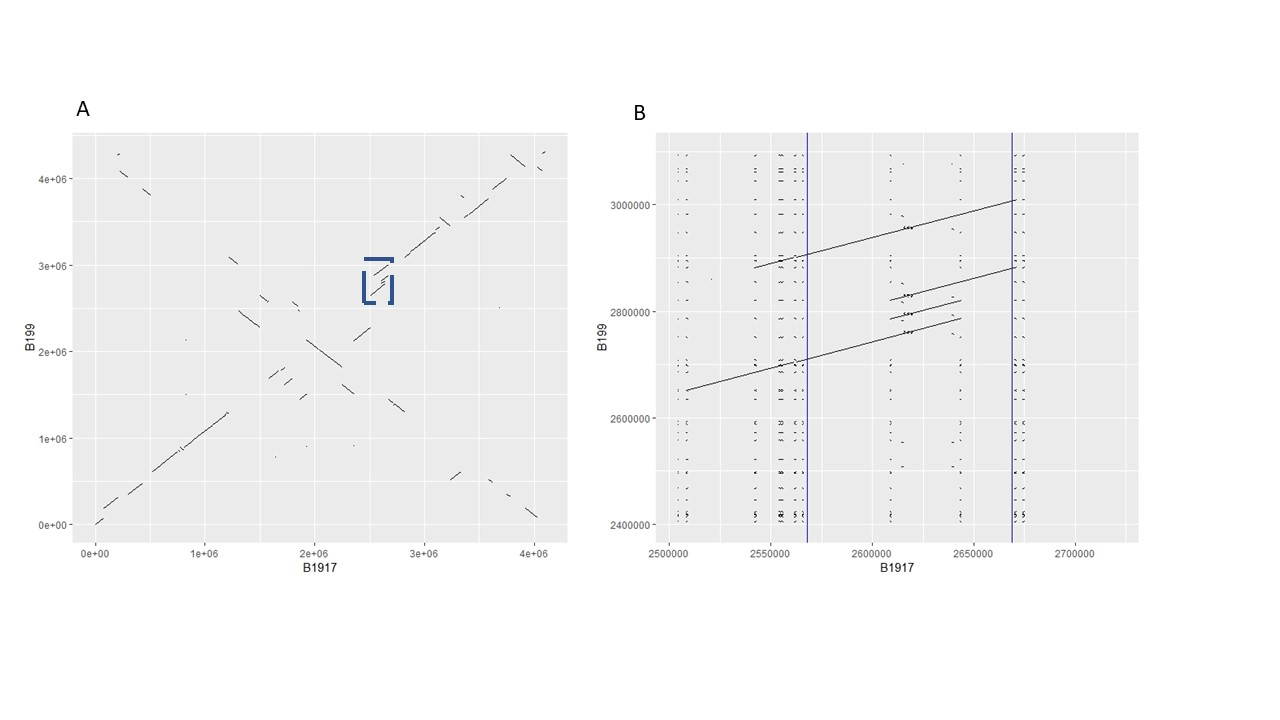
\includegraphics[width=\textwidth{}]{Chapter_1/b199.jpg}
\caption{The genome of B1917(X) compared to strain B199(Y) (A). The section that has a resolved duplication is highlighted in the blue box and expanded in (B). It can be seen that the DNA corresponding to ~2.54Mb to ~3.67Mb on B1917(X axis) has a complex arrangement of duplications. The  CNV estimate by CNVnator is highlighted using blue bars (for start and end positions).}
\label{fig:B199}
\end{figure}


\begin{figure}[h!]
\centering
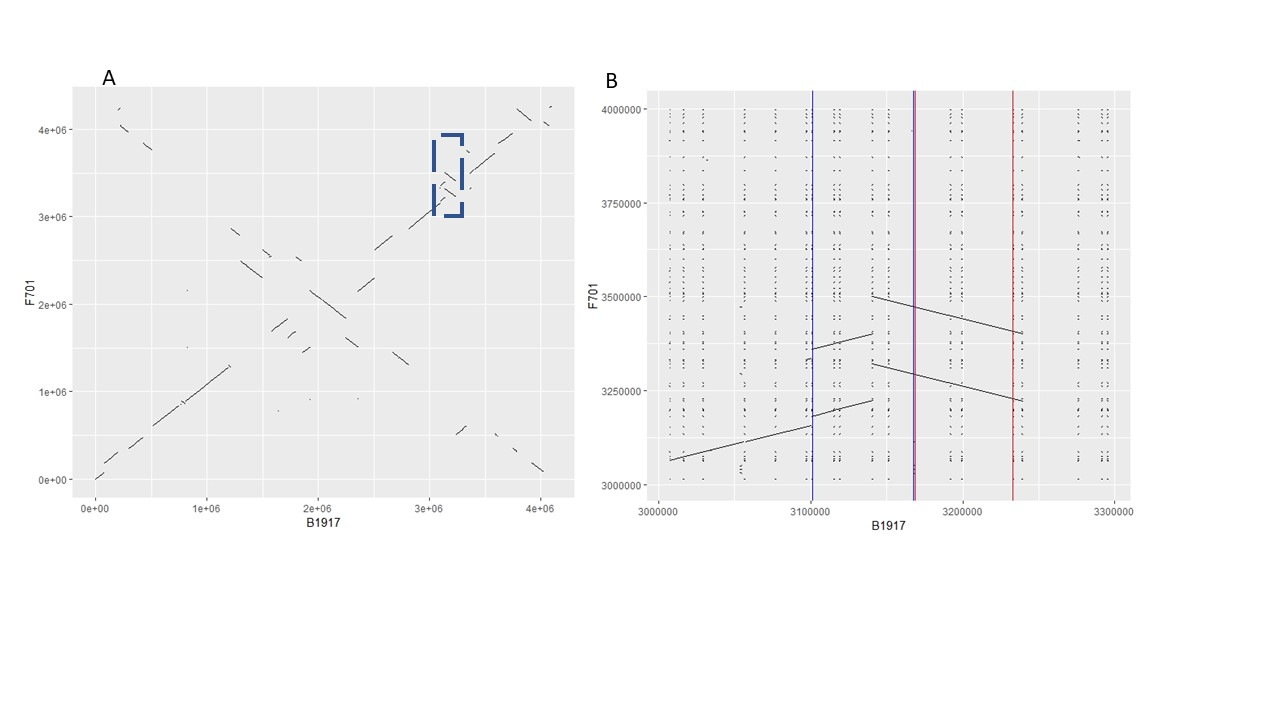
\includegraphics[width=\textwidth{}]{Chapter_1/f701 new.jpg}
\caption{The genome of B1917(X) compared to strain F107(Y) (A). The section that has a resolved duplication is highlighted in the blue box and expanded in (B). It can be seen that the DNA corresponding to ~3.1Mb to ~3.24Mb on B1917(X axis) is duplicated in F107 but that partway through it has been disrupted by an inversion. The two CNV estimates by CNVnator are highlighted using two coloured bars each (for start and end positions).}
\label{fig:F701}
\end{figure}

\subsection{274 CNVs fell at 11 `hotspot loci'}

\subsubsection{Cohort statistics}

The pipeline was applied to predict CNVs in 2709 B. pertussis isolates for which short-read sequence data was available in the Sequence Read Archive (SRA) or locally provided (n=94). Of the 2709 total B. pertussis samples, 94 exhibited < 30x average coverage and 185 had high read coverage noise. Therefore, the final dataset included 2430 B. pertussis isolates. Due to its size this dataset was dubbed the `large cohort dataset' and is reffered to as such throughout the thesis. 

Of the 2430 studied isolates, 1711 had all genes predicted at single copy and therefore did not make any further appearances in the analysis. This confirmed that B1917 had a highly representative gene complement as these 1711 isolates contained all of the genes present in B1917 at single copy. This left 719 strains with at least one deletion or CNV. Of the 719 strains with CNVs: 191 isolates contained 273 CNVs as some isolates contained multiple CNVs. In summary, therefore, 7.8\% of the studied BP strains contained at least one CNV.

The copy number estimates (Figure \ref{fig:Heatmap}) were plotted as a heatmap which demonstrated that CNVs were frequently found at particular loci, which I termed ‘hotspot’ loci.  

A visual analysis of this data revealed that the key results observed in the manually resolved dataset are confirmed in the global cohort of 2709 B.pertussis strains, namely: CNVs clustered at specific loci;varying gene content within these clusters and a many long CNVs (\ref{fig:Heatmap} and \ref{fig:Network_1_heatmap}).





\subsection{Hotspots}


CNV hotspots are found in a diversity of organisms, including bacteria, animals and plants. In-depth analysis of hotspots is, however, rare. This may be due to the complex nature of CNVs in comparison to SNPs- A single nucleotide mutation can be represented easily in a simple format (for example as a wildtype or non-wildtype base or reference base and observed base(s) ) whereas CNVs are a much more organic and dynamic mutation type. Their composition and copy number is highly variable. Whilst visual inspection showed that CNVs fell primarily at the same set of approximate locations (Figure \ref{fig:Heatmap}),  further description of this phenomenon was limited without more sophisticated analysis. I was therefore motivated to create a generic quantitative framework in which CNV hotspots could be analysed.

\subsubsection{Using network graphs to analyse hotspots}

In microbiology,  trees are frequently used to compare differences (normally SNPs) in a DNA sequence that is shared between multiple individual strains (the core genome), yet trees are a generic concept and form part of the mathematical field of graph theory. A tree is a type of graph in which all elements are related to one another other, in this case by sharing the same core genome DNA. Graphs are constructed using nodes and edges, which represent data points and relationships, respectively. A phylogenetic tree aims to quantify the relationships between the datapoints (isolates) by creating the simplest graph that explains the observed DNA patterns.

% In a tree based on core genome SNPs all samples in the tree are comparable because they being compared on a shared trait-the core genome. The tree structure therefore could be easily adapted to compare, instead of strings of DNA, strings of single copy or 0 copy (coded as 0's) and 2+ copy genes (Coded as 1's) (Figure \ref{fig:All_data_hclust}) across the studied cohort of 2000+ BP strains. All isolates would therefore be compared, on gene copy number, similar to a pan-genome study. Whilst this is interesting, its usefulness is limited for analysing the dynamics of CNVs within a hotspot as strains may have multiple duplications in different hotspots. As trees are a specific type of graph, however, a more generic type of graph was applicable- a network graph.


% \begin{figure}[h!]
% \centering
% 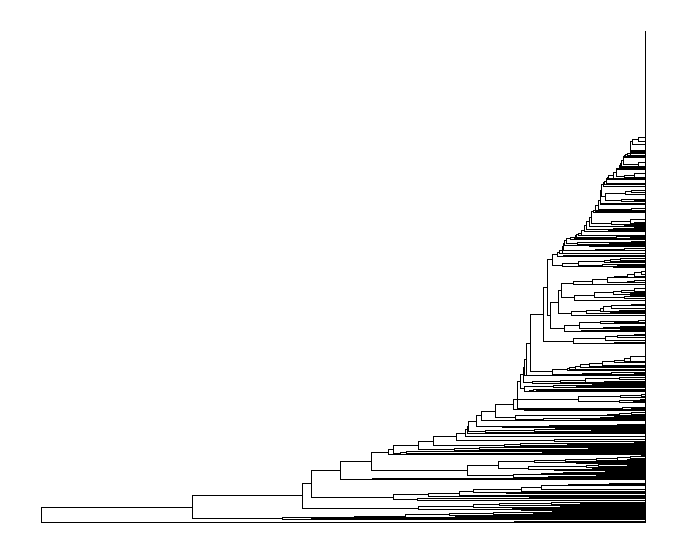
\includegraphics[width=\textwidth{}]{Chapter_1/Rplot140.png}
% \caption{A tree based on the copy numbers of all 720 BP isolates which had at least one gene with a CNV.}
% \label{fig:All_data_hclust}
% \end{figure}

In order to create the network graph, the relationship between all CNVs was quantified as the proportion of gene content overlap between all pairwise comparisons. Network graphs were constructed between CNVs (‘nodes’) that overlapped with each overlap coded as a line (‘edges’). The 273 identified CNVs formed 24 network graphs, representing 24 distinct genomic loci (Figure \ref{fig:Networks_all} & Table \ref{tab:Network_table}). Only 11 network graphs, corresponding to the hotspot loci, included three or more isolates and contained 254/273 (93\%) of the predicted CNVs. Once the data had been coded as a simple network of overlapping CNVs a whole array of analyses was possible.

\begin{figure}[h!]
\centering
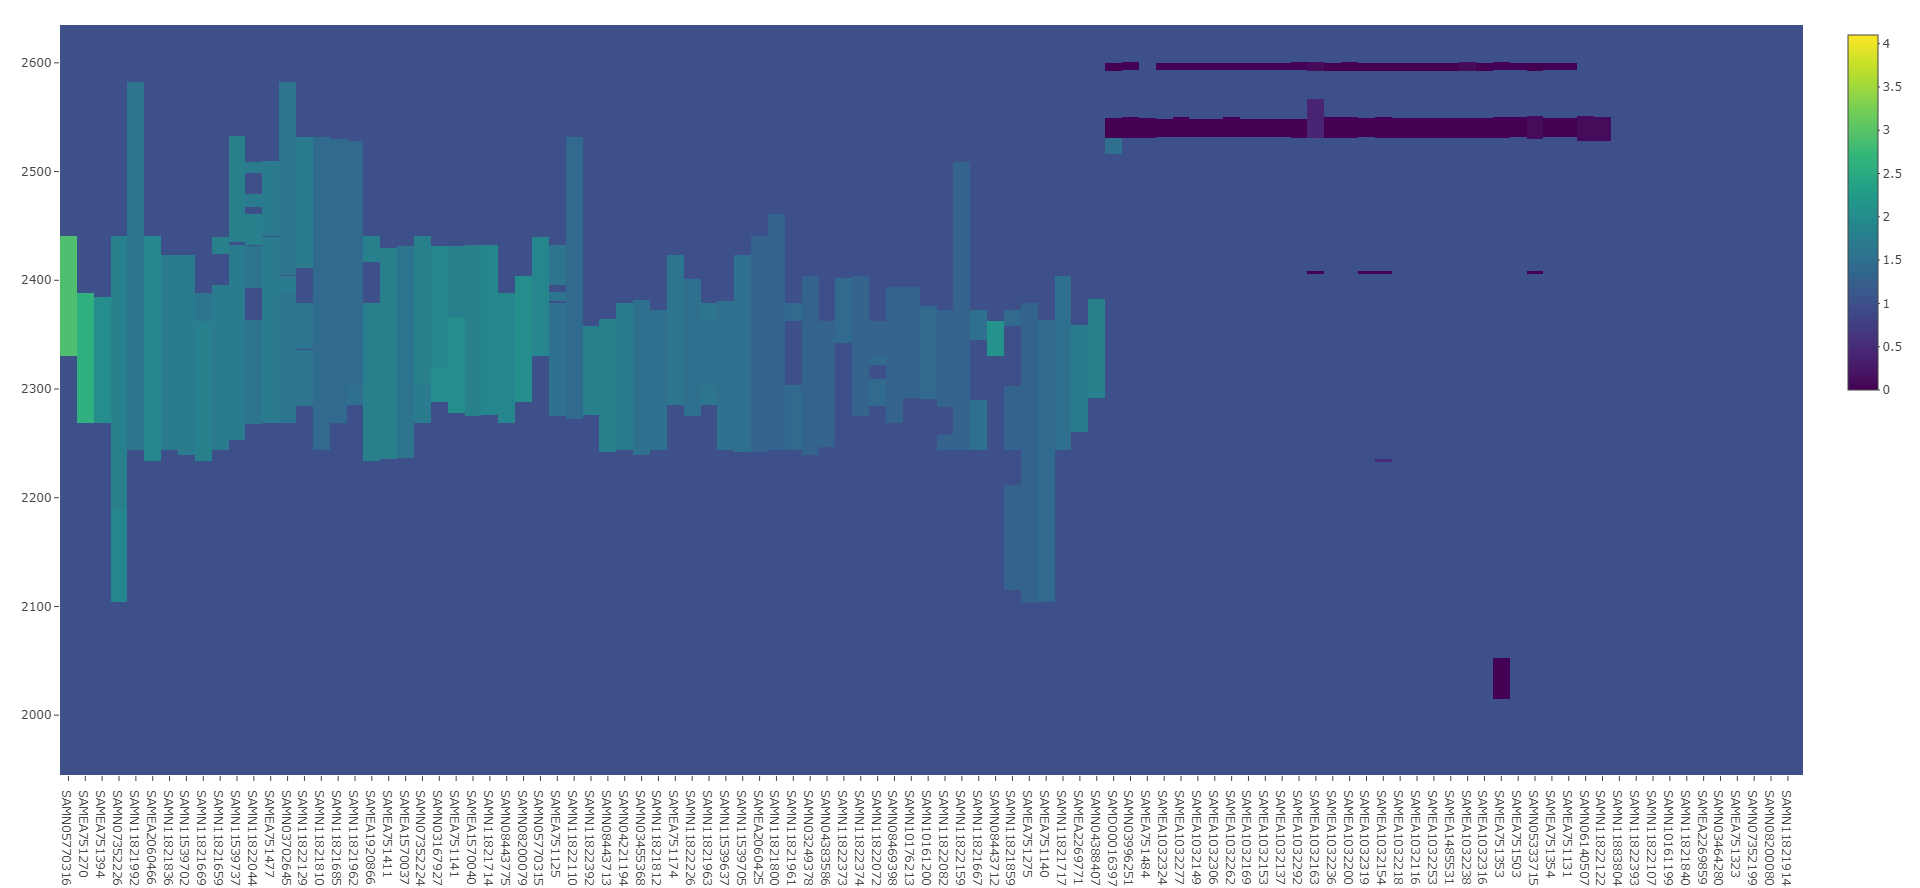
\includegraphics[width=\textwidth{}]{Chapter_1/heatmappy.png}
\caption{ A section of the heatmap comprising the majority of CNVs in Network 1, including a triplication of this locus. Isolates are in columns, while rows indicated the index of each gene in the reference sequence. The colour scale (Z axis) indicates the copy number of each gene. A legend of the colour scale is on the far right.}
\label{fig:Network_1_heatmap}
\end{figure}

\begin{figure}[h!]
\centering
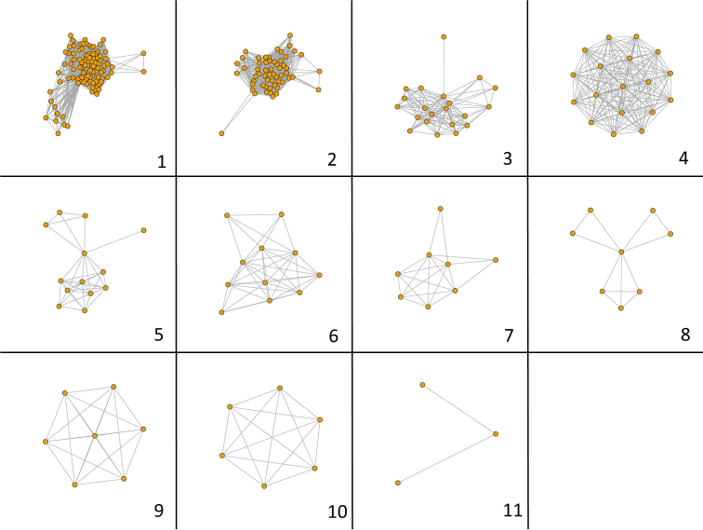
\includegraphics[width=\textwidth{}]{Chapter_1/Networks all.png}
\caption{ 11 networks of 3 or more overlapping CNVs were detected.}
\label{fig:Networks_all}
\end{figure}

\subsubsection{Using the power of networks to leverage new data }
Once CNVs are within a network structure, in-depth analyses can be undertaken. One of the most interesting questions that can be answered using networks was to what extent did CNVs within each hotspot overlap with one another. This is known as network density- the percentage of theoretically possible edges observed between nodes in a network. The mean density of all CNV networks was 71\%, indicating that, overall in the dataset, the CNVs in each network were highly interconnected. This strongly indicated that the networks were composed of CNVs which not only overlapped with one other CNV in the network (as was the minimum permissible criteria for membership to a network), but frequently overlapped with the majority of CNVs in a network. The network density was variable, however (Table \ref{tab:Network_table}).

Further to calculating the network density it was apparent from a visual inspection of the heatmap that some networks were more tightly clustered around a central point than others (Table \ref{tab:Network_table}). This feature could be quantified using the structure of networks and may reveal aspects of the underlying biology of CNVs in BP. Networks were investigated to identify which genes formed the ‘core’ of the network. It was hypothesised that most networks would centre on a small group of genes, as can be visually seen in the heatmap (Figure \ref{fig:Heatmap}). To define the network core, I determined the genes contained in at least 55\% of the >1 copy genes in each network. 

\begin{figure}[h!]
\centering
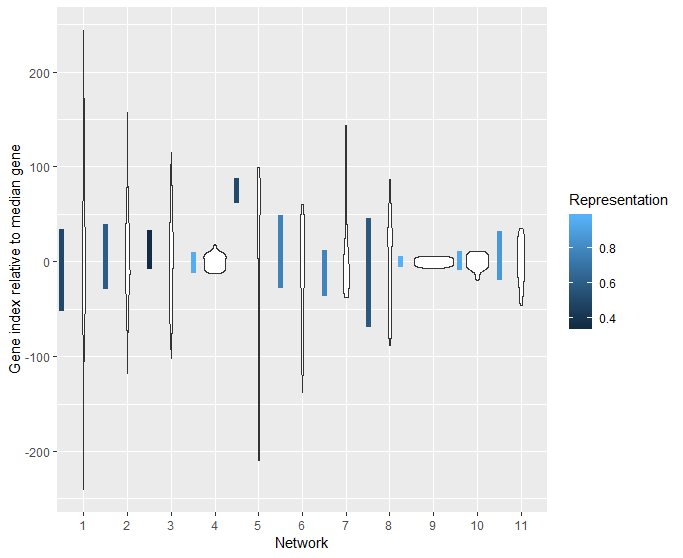
\includegraphics[width=\textwidth{}]{Chapter_1/Rplot135.png}
\caption{ The distribution of CNV genes in each network were plotted in relation to the median gene in the network as a violin plot. For each network the core-CNV range was plotted to the left of each violin. How representative the core-cnv was of all the genes in the network is displayed as a colour gradient.}
\label{fig:Core_rep}
\end{figure}



To contextualise this data , the difference between the central core and the mean CNV length within each network (analogous to the core and accessory genome in the study of pangenomes) was quantified-this formed the core representation statistic (Figure \ref{fig:Core_rep}). This revealed that the core of most networks, with the exception of network 3, comprised at least 50\% of the mean CNV length  in each network. Thus, this supports the network density statistic as  10 of the 11  hotspot loci described here were composed of CNVs that varied around a central core rather than overlapping CNVs arranged in series.  Similar to network density, how much of the average gene content of the network was made up by the core varied between networks (Table \ref{tab:Network_table}).

A number of network cores contained genes with varied predicted functions and as network cores represented 50\% of the CNV genes within most networks, it is logical that CNVs containing these cores shared similar phenotypes. For example, Network 1 contained genes for flagellar motility ; Network 2 contained the nuo operon which is linked to respiration and Network 3 contained the fim3 gene involved in the pathogenesis of B. pertussis and present in some acellular vaccine formulations.

In addition, the networks contextualised the 25 resolved genomes previously studied, the majority of which were in networks 1, 2, and 3.


\begin{table}[]

\resizebox{\textwidth}{!}{%
\begin{tabular}{|l|l|l|l|l|l|l|l|}
\hline
Network name & Frequnecy & Mean length (genes) & Median start gene & Median end gene & Mean copy number & Core proportion (\%) & Network density (\%) \\ \hline
1 & 102 & 106 & RS12140 & RS12755 & 1.6 & 50 & 55 \\ \hline
2 & 57 & 82 & RS15100 & RS15490 & 1.7 & 61 & 63 \\ \hline
3 & 21 & 80 & RS07175 & RS07660 & 1.68 & 35 & 60 \\ \hline
4 & 18 & 20 & RS00010 & RS00130 & 1.35 & 96 & 100 \\ \hline
5 & 13 & 67 & RS19230 & RS19625 & 1.93 & 51 & 50 \\ \hline
6 & 11 & 75 & RS05505 & RS05935 & 1.6 & 77 & 73 \\ \hline
7 & 8 & 49 & RS04185 & RS04430 & 1.88 & 78 & 71 \\ \hline
8 & 8 & 74 & RS09665 & RS10290 & 1.82 & 58 & 43 \\ \hline
9 & 7 & 13 & RS19965 & RS10580 & 2.49 & 98 & 100 \\ \hline
10 & 6 & 23 & RS19465 & RS19565 & 1.32 & 94 & 100 \\ \hline
11 & 3 & 45 & RS01035 & RS01300 & 1.63 & 87 & 67 \\ \hline

\end{tabular}%
}
\caption{Table of network statistics}
\label{tab:Network_table}
\end{table}



\subsubsection{qPCR verification of a duplication}
In order to validate the CNV predictions, a CNV was chosen for further analysis. The initial verification method was undertaken by qPCR  but later verification was achieved by Nanopore sequencing, which forms a substantial amount of work described in Chapter 2. It was therefore necessary to choose a CNV with a tractable size  that could fit, in its full tandem configuration, into an ultra-long Nanopore read. The genome of UK54 (SAMEA1920853) was predicted to have a 16 kb long CNV at a copy number of 4; short enough to observe the CNV locus in a single sequence read on the Nanopore platform, assuming that each copy occurred in tandem as observed in both our data and previous reports. This was the highest copy number CNV in the dataset. The duplication was part of Network 9 which was comprised of 7 other duplications, one of which was also predicted at a copy number >2  (3.3, Strain SAMN11822098).

The copy number of this locus in UK54 was validated using qPCR to ensure the copy number prediction was correct.

A probe and primer set (table x) was designed to quantify the DNA copy number of a DNA segment inside of the duplication and outside of the duplication, using a delta delta CT analysis. This method is most often used to quantify the changes in the expression levels of genes, but is equally suited for quantifying the DNA itself, rather than RNA in a RT-qPCR.

The optimum concentration of X and Y(table x) was found and the experiment could be conducted.


The relative copy number of a gene within the CNV compared to a single-copy gene encoded outside the CNV locus was 4.38 +/- 0.4 which matched the read depth-based prediction.

While one predicted CNV had been verified, verification was not practicably feasible for the remaining 273. I therefore sought to verify CNVs in an alternative way.

\subsubsection{Predicted CNVs are highly associated with repeats}

Verification was possible by investigating the association of predicted CNVs with repetitive elements in comparison to all genes. All previously published and resolved CNVs were adjacent to repetitive sequences, suggesting this was a clear marker for true CNVs. Only CNVs occurring in isolates which had closed genomes (excluding those in the manually resolved dataset) were analysed as IS content differs between isolates and repeats not resolved in fragmented assemblies. This left 16 CNVs in 13 isolates remaining.

The 16 predicted CNV boundaries were significantly (p<6-08) closer to repeat genes (median distance of +/- 1 gene) than non-CNV genes (median distance of +/- 5 genes) (Figure \ref{fig:CNVs_close_to_repeats}). This, in conjunction with our stringent quality control steps and the previously accurate predictions, supports the accuracy of the prediction of 274 CNVs.

\begin{figure}[h!]
\centering
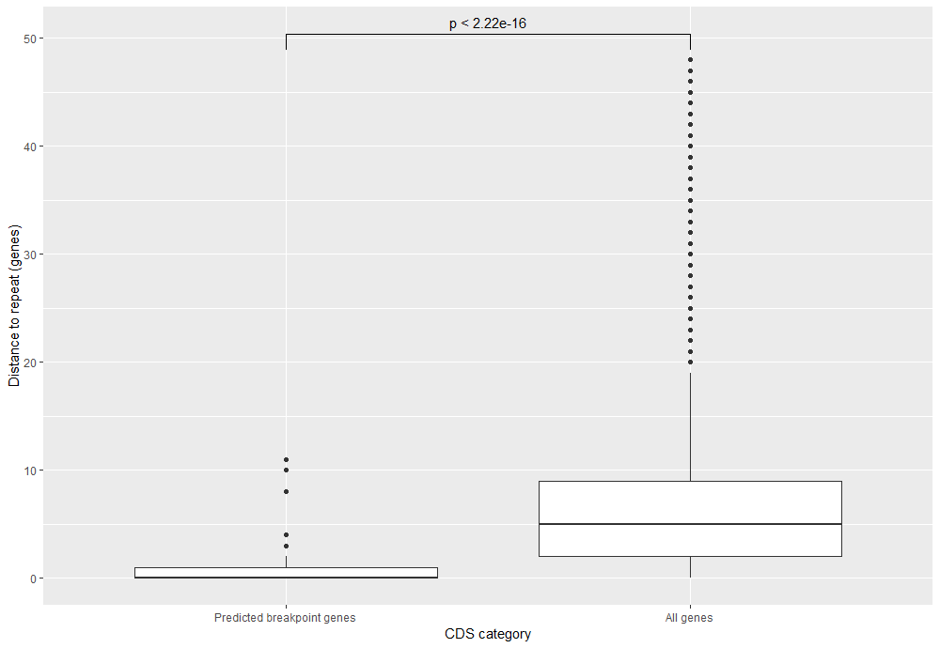
\includegraphics[width=\textwidth{}]{Chapter_1/Picture1.png}
\caption{The distance (measured in genes) between CNVs and repeat genes was identified in closed genomes. The ends of CNV loci were found to be significantly closer (median: 0 genes) to repeats than the average gene (median: 5 genes).}
\label{fig:CNVs_close_to_repeats}
\end{figure}

\subsubsection{CNVs occur sporadically throughout the phylogenetic tree}
It was demonstrated that while CNVs did overlap at hotspot loci they often had unique gene contents-strongly indicating each arose from an independent mutation. Therefore, I hypothesised that there was no strong phylogenetic relationship between CNVs within a network. To test this, we sought to estimate for each network if at any point in the phylogenetic tree an ancestral strain, represented by an internal node of the tree, was likely to have had the corresponding CNV (Table \ref{tab:ASR_table}). This was performed by using presence or absence of CNVs within a network as a discrete trait.


\begin{table}[]
\resizebox{\textwidth}{!}{%
\begin{tabular}{|l|l|l|l|l|l|l|}
\hline
Node Alias & Network name & Node ID & Node depth (from tip to root) & Maximum distance to tips (branch length) & Maximum distance to tips (SNPs) & Known false positive \\ \hline
1 & 1 & 341 & 3 & 0.000703 & 3 & Y \\ \hline
2 & 1 & 536 & 2 & 0.000469 & 2 & Y \\ \hline
3 & 1 & 544 & 8 & 7.03E-04 & 3 & N \\ \hline
4 & 1 & 582 & 3 & 0.000234 & 1 & N \\ \hline
5 & 1 & 583 & 2 & 0 & 0 & N \\ \hline
6 & 1 & 1272 & 2 & 0 & 0 & N \\ \hline
7 & 1 & 1455 & 2 & 0 & 0 & N \\ \hline
8 & 2 & 310 & 2 & 0.00E+00 & 0 & N \\ \hline
9 & 2 & 584 & 2 & 4.69E-04 & 2 & Y \\ \hline
10 & 2 & 906 & 2 & 0.000234 & 1 & Y \\ \hline
11 & 2 & 960 & 3 & 0.000234 & 1 & Y \\ \hline
12 & 2 & 1210 & 2 & 0 & 0 & N \\ \hline
13 & 4 & 137 & 5 & 0.001642 & 7 & Y \\ \hline
14 & 5 & 399 & 2 & 0.000234 & 1 & N \\ \hline
15 & 5 & 1435 & 2 & 0.000938 & 4 & N \\ \hline
16 & 9 & 802 & 2 & 0 & 0 & N \\ \hline
\end{tabular}%
}
\caption{Table of ancestral reconstruction results}
\label{tab:ASR_table}
\end{table}

Ancestral state reconstruction (ASR) resulted in 16 nodes near the tips of the tree (<=7 SNPs and <=8 tree splits) having a high likelihood (>0.8 empirical Bayesian posterior probability) of being in a duplicated state. Due to the large number of isolates studied in combination with the extremely low diversity of B. pertussis, however, branch lengths were often 0- potentially skewing the results. Further investigation of this effect showed that 7 of the 16 nodes of interest had just one tip with branch length 0 directly stemming from the node. The extremely close relationships between these tips and nodes leads to an overwhelming statistical signal to the ASR algorithm leading to false positive results. These 7 nodes were ignored (noted in Table \ref{tab:ASR_table} as `Known false positives'). Our results therefore indicated very limited heritable of CNVs, but yielded 8 putative examples of the mutation being maintained over small evolutionary time scales.

\section{Discussion}

B. pertussis is described as a monomorphic bacterium that has evolved as a human-specific pathogen through gene loss via homologous recombination between direct repeats. However, homologous recombination can also cause multi-gene CNVs. Although 12 multi-gene CNVs had been described previously, no systematic analysis of CNVs in B. pertussis had been carried out. In this chapter, short-read genome sequence data generated on the Illumina platform for 2430 strains was analysed using read depth as a proxy for copy number.  The results revealed 11 clusters consisting of 273 CNVs, some of which comprised hundreds of genes, revealing a novel aspect of genetic variation among B. pertussis. This contributes to a growing literature that demonstrates that quantifying B. pertussis diversity requires a comprehensive view of mutation types, not just the quantification of DNA base changes.

%Studying genetic mutations in a holistic way by incorporating structural variations as well as nucleotide changes is well established in eukaryotic organisms but is often not undertaken in prokaryotes. 

\subsection{Manually resolved dataset}

\subsubsection{Dataset construction and evaluation}
%Our data was really good.
Analysing read depth data for the presence of CNVs is an indirect method of finding CNVs and as such its use carries its own inherent strength and weaknesses. To quantify this, estimates were compared to a set of known CNVs.

A set of 28 isolates which had been sequenced by a combination of Nabsys, Pacbio, Illumina and OpGen optical mapping provided an excellent set of known CNVs in BP. The goal of the method presented here was to predict these CNVs using read depth signals from short read data alone to simplify the process of screening for CNVs. 

The dataset fell into three groups: ideal for analysis (n=24); not ideal for analysis (n=2) and poor quality (n=1). Two genomes with complex CNVs were separated into the `non-ideal' group as their complex nature meant that read-depth was theoretically under-powered to predict these CNVs.  A single genome failed quality control tests (low read depth noise and >30x coverage) and was excluded from further analysis. 

%The strengths and weaknesses of this analysis were assessed based on its performance of these three groups.

It was not possible to express the results of this comparison experiment formally as sensitivity and specificity because a true CNV could be predicted correctly (at a minimum 80\% reciprocal overlap) but a false positive also predicted for that CNV (for example at 20\% of the length of the CNV) . This therefore meant that a contingency table where each element of the test (here a CNV) could only fall into one category (true positive; false positive; true negative or false negative) was not suitable. This also meant that whilst one true negative was simulated here, it was not directly comparable to the true positives. 

Establishing true negatives from real data was not carried out as it was not possible to verify that the high levels of scrutiny that were applied to the true positives was applied to these `true negatives'. This is especially true given that 16 CNVs were predicted in publicly available closed genomes which  appeared to have the hallmarks of true CNVs. 

By varying the window length in response to the read depth noise of each sequencing sample the appropriate analysis was conducted for each genome therefore overcoming the hurdle of inter-sample read depth noise by providing a demonstrably accurate set of duplications in BP. However, there was limited chances to test this methodological step as the manually resolve dataset was of a generally high quality. The most important result this enabled was the study of 1000's of bacterial isolates of varying quality generated using a variety of different parameters. This is a scale of CNV prediction in prokaryotes that is not often achieved, likely due to high false positive predictions. 


\subsubsection{Low false positives and low false negatives but slight over-specificity}
%Big up the pipeline. it performed really damn well

A considerable strength of the pipeline was the low rate of false positives and false negatives. Out of the 24 CNVs which were judged to be highly suitable for this analysis, 23 had the correct CNV predicted (95\%), as defined here by a strict minimum 80\% reciprocal overlap.  An 80\% reciprocal overlap is superior to many published methods which define a correct prediction as only a minimum 50\% overlap between a predicted and true CNV to be sufficient for a prediction to be considered correct. There was, however,  one false negative and it was unclear why this CNV had been failed to be predicted in this case.  Overall, It was demonstrated that this method was comparable to many studies.

A small number of false positives were predicted. Of the 24 highly suitable CNVs,  3 (13\%) of these CNVs were predicted as two CNVs : a major fragment and a minor fragment. In these 3 cases the major fragment was big enough to satisfy the reciprocal overlap rule and so therefore the true CNV had been adequately predicted. The three minor fragments were considered false positives. It is therefore likely the pipeline is slightly too specific, given that the vast majority of the predictions were highly accurate. The balance of sensitivity and specificity was balanced through testing various window lengths and the impact this had on the mean over the standard deviation of read coverage which was optimised for each sample to be between 4 and 5 (cite CNVnator). It could be that there are extra heuristics or noise-smoothing tools that can reduce the over-specificity of this analysis by further tweaking the window length.  The current over-specificity of the method is likely to inflate the number of CNVs predicted in the large cohort analysis. 

%Extra noise smoothing tool: https://www.ncbi.nlm.nih.gov/pmc/articles/PMC6196408/

A false positive CNV was predicted at a second locus in the x sample. The existence of a CNV was investigated in this isolate and whilst both PacBio and Illumina showed a moderate rise in coverage at this locus, optical mapping and Nabsys data did not corroborate a CNV present at the locus. It is therefore unclear exactly what was causing this rise in coverage, but it may have been due to a mixed population of cells (see Chapter 2). The aim of this dataset was to evaluate this pipeline in the most conservative way and therefore this result was counted as a false positive, despite mixed evidence that it was a CNV.

\subsubsection{The method has high breakpoint accuracy}
%Breakpoint accuracy
The predictions were also highly accurate, having a median distance of 0.5 genes to their true start/end.

There were however, many predictions that had considerably worse breakpoint accuracy. Two of these estimates were related to the over-specificity of the pipeline leading to a CNV being correctly predicted but ending a large distance before the true CNV end. This data also corroborates that this method is slightly over-specific.

It is to be expected, therefore, that the CNVs predicted in the larger cohort of BP isolates would generally be highly accurate.


\subsubsection{Indirect evidence of breakpoint accuracy from novel predicted CNVs}

Beyond the 28 isolates with known CNVs, an indication that the predictions were accurate was found in the analysis of the global cohort of isolates. The mechanism that previously discovered CNVs are generated by in BP is by homologous recombination between large repeats and therefore, true predictions should be flanked by such repeats. I found that the breakpoints of these predicted CNVs were significantly closer to insertion sequences (median: 0 gene) than the majority of genes in the genome (median 5 genes). The closer association of CNVs to repeats indicates the predictions are true, rather than a spurious result with no association to the underlying biological processes that are known to cause such mutations. As this evidence is indirect, however, this association could be caused by a different mechanism which is as of yet, unknown. 

In Chapter 2, additional direct and indirect evidence of CNVs is provided. The best source of direct evidence of CNVs is by capturing whole CNV arrays in single long sequencing reads, but failing that, long reads can also provide indirect evidence of CNVs. Indirect evidence can be obtained by searching long-read data for sequences which spanned the end of one copy of the tandem duplication and the start of the second copy (Junction sequences). 


\subsubsection{Copy number discrepancy}
An interesting feature of read-depth mapping is that the read-depth is an amalgamation of information from many different cells in the population that was sequenced (Figure \ref{fig:CDC_copy_number_discrep} ). Whilst this appears to be erroneous, it was key to the work in Chapter 2 and was one of the driving forces that led to the investigation of mixed populations of cells. It is evidenced in Chapter 2 that CNV instability is likely to account for many of these `intermediate' copy number estimates.

The accuracy of the copy number prediction was demonstrated by qPCR  which verified the copy number of a CNV in UK54. UK54 was chosen as it contained the highest copy number CNV in the dataset and was therefore an attractive option for qPCR, which can struggle with quantifying changes of a two fold difference (e.g between single and double copy regions). The qPCR resulted in a prediction of 4.4 +/- 0.4,  verifying the predicted copy number of 4. The accuracy of qPCR to determine intermediate copy numbers, however, is limited but could be achieved with increased technical repeats which would give tighter upper and lower bounds.



\subsubsection{A failure to resolve complex CNVs}
The biggest weakness of this method stems from an inherent weakness of read-mapping. It was found that it is not possible to correctly resolve complex CNVs. Other information from short read sequencing can theoretically be used to identify SVs, because they form primarily by homologous recombination between repeats  (~1kb) which exceed the read length (<=300bp), this data was demonstrably absent at an CNV locus  (Figure \ref{fig:Close_but_no_cigar}). Therefore for screening CNVs using short read data, read-depth is the only appropriate signal for BP.

A complex CNV, such as the two CNVs in the manually resolved dataset which had inversions in addition to duplications, is beyond the resolution of read-depth based approaches and as such were judged to be `not-ideal' for CNVnator to predict. In order to examine how complex CNVs are interpreted by CNVnator, these two isolates were analysed separately. The CNV in the B199 strain was composed of nested CNVs arranged in an extremely complex way whilst in F701 there was a CNV disrupted by a small genomic inversion compared to the reference B1917 sequence. 


 When CNVnator was used to predict these CNVs, none of the results shared an >=80\% reciprocal overlap with the individual true results and therefore the true CNVs in these isolates were not predicted correctly. However it is notable that the approximately right region had been interpreted as a CNV. However, even merging the CNVs into a single unit did not enable the predictions to pass the strict reciprocal overlap threshold. An additional problem was that the isolate F701 had been predicted as two separate but adjacent CNVs which indicates over-specificity (see below).

These results highlight how challenging it is to predict complex CNVs using read depth alone. It is likely that in the large cohort dataset that a number of CNVs would be complex and therefore have reduced breakpoint accuracy in addition to the predictions masking a more complex arrangement.Whilst F701 had a small inversion, it is likely that some isolates in the larger dataset would have been disrupted by larger inversions and therefore be predicted as two CNVs that are distant on the B1917 genome but may be contiguous on the CNV isolates.  This effect may have inflated the number of CNVs predicted and the basis of future work could be to resolve many of these isolates using long read technologies. Whilst the ultimate goal of long-read sequencing is to generate a closed genome that truly encompasses all CNVs, current platforms and analysis appear to not be adequate to generate consensus sequences with large CNVs in (Ring et al +chapter 2). However, at a minimum, long read assemblies with collapsed repeat regions would determine the gene order of simple CNVs and any spurious CNV predictions could be investigated further.




\subsubsection{Pipeline conclusions}
In order to accurately evaluate the methodology the true positives , the false positives and the breakpoint accuracy were judged in relation to the dataset as a whole, minus the low quality genome (27 CNVs). This is in recognition that the large cohort analysis was composed of isolates that also passed quality control tests but that there was no knowledge of which CNVs are complex/disrupted by inversions. 

Taking all the results of the comparison into consideration, the most conservative statistic is that 74\%(20/27) of CNVs of adequate quality were correctly predicted with excellent breakpoint accuracy. 

In the results and discussion,however, this statistic was explored and it was found that 3 extra CNVs were predicted as a correct (satisfying overlap rules) major fragment  but also generated false positive minor fragments. Therefore, a less conservative statistic is that 85\% (23/27) of CNVs were correctly predicted. Despite these highly accurate predictions, complex CNVs were very had to predict.




\subsection{Analysis of CNVs in a large cohort of B.pertussis}


\subsubsection{Theoretical hurdles in analysing `hotspot' loci}

%Bad study which just merges CNVs based on a 1 bp overlap
%https://www.nature.com/articles/s41598-017-14768-0#Sec8

%Well established CNV networks paper
%http://repository.ias.ac.in/111042/1/journal.pone.0066843.PDF
It was readily apparent from the heatmap (Figure \ref{fig:Heatmap}) that CNVs fell at specific loci. It was impossible, however, to adequately describe this phenomena using this data alone. Whilst network graphs overcome this problem, it was a considerable theoretical hurdle to overcome, considering that network analysis of CNVs is almost non-existant in the literature. Retrospectively searching for publications which utilise network graphs to analyse the spatial organisation of CNVs returned only one methods paper (detailing the bioinformatics tool HD-CNV) with a modest number of citations (15 as of 27/01/2019). Many of these studies utilised HD-CNV to simplify their CNV calls in eukaryotes to a non-redundant set of regions that experienced frequent CNVs, but went no further in analysing the composition of these networks. As CNVs are a ubiquitous feature in all kingdoms of life, using networks to analyse CNVs is an is a flexible and generic framework to analyse the poorly described phenomena of CNV hotspots.

An advantage of using networks to describe hotspot loci was the ability to semantically categorise CNVs to unite the findings of many studies and contextualise them with new data. Previously, using limited data, a ‘hotspot-like’ effect had been demonstrated by resolving four CNVs with subtle gene content variations at the same loci corresponding here to Network 1, at which other CNVs had also been reported. This is contextualised both by the dataset of 24 high quality manually resolved CNVs (Figure  \ref{fig:CDC_breakpoint}) and the results from the BP cohort which provided another 90 CNVs at this location.


%Quantifying that the vast majority of CNVs fell at hotspot loci was evidence that CNVs may be formed primarily by selective amplification of the core genes may be under selection yielding multiple independent mutations.


\subsubsection{How hotspots may have been effected by weaknesses of the pipeline}

It was demonstrated that the pipeline was overspecific, thus leading to some CNVs predicted as multiple fragments in addition to a number of predictions to stop short of the true CNV end. This had the potential to impact how the data were interpreted.  It is possible that there this fragmentation causes an inflated number of CNVs to be predicted. I examined how this might have a knock on effect to how CNVs were analysed as networks.



%Network density would be inflated, If each CNV was split up into 3
Fragmentation of CNV calls was unlikely to significantly effect the network density statistic, under the assumption that CNVs were split into fragments separated by small numbers of genes, as was observed in two cases ( 8\% ) of the `high suitability' dataset. This is also under the assumption that splits dont fall directly on regions which are CNV start/end points in other CNVs, which appeared true (Figure \ref{fig:Heatmap} and Figure  \ref{fig:Network_1_heatmap}). Whilst each extra fragment would increase the total number of possible connections in the network, under these assumptions each of the new fragments would inherit all of the overlaps of the true CNV by the same amount and therefore the network density would be unaffected.

In a similar way, core-network representation would be unaffected, apart from by those genes which are single copy inbetween fragmented predictions. The core network statistic was generated by taking the genes that were contained in 55\% of the genes in CNVs within a network. Therefore this statistic was independent of the number of CNVs and instead dependent on the gene content of the CNVs.



\subsection{Is the pattern of CNVs driven by selection?}

\subsubsection{What core regions may indicate about selection}
%Cores are interesting. Conserved core could mean that those CNVs
By using the core-CNV and mean overlap statistics it was demonstrated that the majority of the 11 networks in our analysis consisted of CNVs which varied around a core set of genes, a trend that was also observed in the dataset of 28 manually resolved genomes. The literature suggests that CNVs, due to their length, are mutations which carry large fitness costs-unless there is a significant fitness advantage to the often accompanying higher gene expression.

The large number of copies of IS481 throughout the B. pertussis genome suggests that a very large number of different genome rearrangements 8 and CNVs are possible. Despite the vast diversity of possible CNVs, however, 94\% of observed CNVs appeared at just 11 hotspot loci. This may be because CNVs can be costly mutations, carrying as much as a 0.15\% fitness cost per 1kb, primarily due to increased gene dosage leading to additional transcription and translation rather than replication of a larger genome. According to this estimate, the larger CNVs observed in this study may carry fitness costs over 30\%. Therefore, unless higher levels of transcribed (non-coding RNA) or translated (proteins) gene products provided a strong selective advantage to overcome such a cost, the CNVs is likely to be selected against.

Similarly, a recent paper by Weigand et al demonstrated that when gene orders were analysed in a large cohort of closed B.pertussis genomes, there were also conserved gene orders despite the huge variety of possible combinations. 


 I suggest that this discrepancy between the potential and observed distribution of CNVs, is an indication that strong purifying selection acts on CNVs in B. pertussis. Whilst this hypothesis is supported in the literature, it is also possible that this is attributable (at least in part) to certain loci having a higher likelihood of mutation. 



% https://www.ncbi.nlm.nih.gov/pmc/articles/PMC319510/pdf/pnas00656-0487.pdf
%Other study https://www.ncbi.nlm.nih.gov/pmc/articles/PMC2865909/
An historic study by Anderson and Roth found that in salmonella, certain regions of the genome experienced higher rates of duplication than others, based on their proximity to rRNA operons. This was confirmed by other studies . However it is unclear how this translates to pertussis, which is replete with repetitive DNA. Further analysis of the work presented here could investigate if the hotspot loci have a denser than average cluster of repeats at the median start and end points.
%I hypothesise therefore, that the pattern of CNVs observed in this analysis was formed primarily by the forces of selection, although it cannot be ruled out that some regions of the genome are prone to higher rates of CNV mutations.


%the function of cores can be investigated
%Humans and apes are known to have regions of DNA that are prone to CNVs. They have such different genomes though and with more folding of the DNA and less selection acting on the genome it is not sup[rising.] These may or may not apply to bacteria.
%https://genomebiology.biomedcentral.com/articles/10.1186/gb-2011-12-5-r52




In order to quantify selection pressures acting on DNA sequences, the most used tool is the dN/dS ratio, the ratio of synonymous(dN) to non-synonymous mutations (dS) which in this case, however, is unapplicable. The unstable nature of CNVs in bacteria, and in particular in combination with the low rate of SNPs in BP, mean that the lifespan of a duplication is much too fleeting to acquire even a single SNP-synonymous or not. This short lifespan was described in the ancestral state reconstruction analysis- hypothesised inheritance of a duplication occurred over a timescale that corresponded to just a few SNPs across the whole genome, in the most pronounced example.


%Discussion point:

%This feature could be quantified using the structure of networks and may reveal aspects of the underlying biology of CNVs in BP

\subsubsection{Potential impacts of CNVs}

One of the most frequent hotspots observed in this study included genes for flagellar motility. Motility has been frequently implicated in the virulence of bacterial pathogens, but B. pertussis has long been regarded as non-motile. However, recent research has shown that motility can be occasionally observed in vitro 34 and flagellar biosynthesis genes are expressed during murine challenge compared to in vitro growth, potentially implicating motility or biofilm formation in infection 45. Duplication at this locus may, therefore, affect the virulence, colonisation, or carriage of B. pertussis in the human population, but the influence may be modulated due to the plasticity of CNVs. Whilst no phenotypic charecterisation of CNVs was undertaken here, the goal of exploring genotype-phenotype links for these mutations is the basis of Chapter 3.

The work contained within this chapter Github (https://github.com/Jonathan-Abrahams/Duplications) is a clear demonstration that large cohorts of bacteria can be effectively studied by this methodology.

\subsection{Applicability outside of B.pertussis}
\subsubsection{BP is not unique-Many species likely have hotspots}
However whilst unusual, B. pertussis is not unique, as its abundance of IS elements ranks in the top 30 in a study of 1000’s of bacterial isolates 51.It is likely that such dynamics are playing out in other species proportional to their IS elements load 47,52.

The unusually high number of insertion sequences within the B. pertussis genome, and their relatively even distribution, likely facilitates the genome-wide distribution of structural variants. Indeed, genomes of related species B. parapertussis and B. holmesii each harbour fewer IS elements and thus exhibit fewer rearrangements 50 and very rare CNVs (M.R. Weigand, unpublished). 

\subsubsection{Comparison to PanX}

%Panx is interesting.
Highlighting the strengths and weaknesses of this analysis, there has previously been a single study that analyses large cohorts of bacteria for CNVs. PanX is primarily a bioinformatics user interface that links up multiple data sources in a intuitive and novel way. In its initial release, the pangenomes of approximately 20 bacterial species were analysed (including B.pertussis), with each species often being represented by 100's of isolates. The use of a pangenome in PanX is markedly different from the strategy presented here where a single reference was used and highlights the strengths and weaknesses of using a pangenome as a reference. 

A clear criticism of the PanX study was that, as it was primarily a showcase of the user interface, no methodology was published on how the data was produced. It can be presumed, however, that the reads from each isolate were mapped to the pangenome. This contrasts with mapping to a single reference, which was undertaken here. 

The benefit of using a single well chosen and representative reference is that the genomic context of the CNVs is preserved. It could be demonstrated in this analysis that B1917 represented common gene orders much closer than Tohama, the highly laboratory adjusted reference isolate. In the PanX study, no genomic context was available. It is possible, armed with the knowledge generated in the analysis here, to find that the flagella operon frequently undergoes duplication using the PanX dataset, but because of the lack of genomic context presented, it is in no way clear that there are large contiguous groups of genes undergoing copy number variation. Furthermore, because of this lack of genomic context, the biology of the genome is also hidden. The insights into CNV hotspots generated here are masked in PanX by the use of a pangenome reference.

Whilst using a pangenome masks the genomic context of CNVs, the benefit is that PanX is not limited to studying genes that just occur in the reference genome. Iin this aspect, the analysis presented here has a weakness. It is noteworthy however, that B.pertussis has a remarkably small accessory genomes, which is characterised by gene loss and no gene gain (apart from a small amount in a common ancestor of all modern isolates) and therefore, for B.pertussis, it is not a major drawback that this part of the genome may be missed in the analysis. For other species with much large accessory genomes, mapping to a single reference is unsuitable and would mask large parts of the accessory genome, which often contains virulence and antibiotic resistance genes.

%Reference Pirate here https://github.com/SionBayliss/PIRATE
In order for the work presented here to be more generically useful for other species with more extensive pangenomes it is likely necessary that reads will need to be mapped to a pangenome, as was likely undertaken with PanX. Future work on this subject could be to identify a linkage metric in order to `re-inject' some genomic context to the pangenome study- it might be found that genes that are co-duplicated in multiple isolates are statistically likely to be contiguous in those isolates. This may provide all the positives of mapping to a pangenome without the significant compromise of loosing genomic context.




\subsubsection{Phylogenetics reveals limited heritability of CNVs}

It is easy to assume that the overlapping networks of CNVs indicate these mutations have been inherited from a common source. However, CNVs are known to be both one of the most frequent mutation types and also highly unstable. I therefore wanted to confirm this by simulating ancestral genotypes based on the observed pattern of CNVs at the tips of the tree using ancestral state reconstruction.

Ancestral state reconstruction was undertaken on the assumption that it was equally likely to gain and lose a CNV. This is a highly reductive model that greatly favours the maintenance of high copy number states. Despite this, ancestral state reconstruction predicted very few events of the inheritance of CNVs. Similarily another assumption that was made was that the CNVs within the same network could be inherited. This is despite the fact that many CNVs in the same network appear so different that they either have a different origin or have undergone extensive secondary SVs to change to a different conformation. This second assumption also favoured inheritance of CNVs   and yet, limited hertiability was found.

Therefore the ASR analysis of the inheritabiltiy of CNVs in BP concur with the  wider literature. CNVs are frequent mutations that are highly unstable , which seem to `appear' and `disappear' on the phylogenetic tree rapidly.



\end{document}



